\documentclass[a4paper]{report}
\usepackage[useregional, showdow]{datetime2}
\usepackage[portuguese]{babel}
\usepackage[T1]{fontenc}
\usepackage{inputenc}
\usepackage{amsmath}
%\usepackage{graphicx}
\usepackage{booktabs}
\usepackage[colorinlistoftodos]{todonotes}
\usepackage[plainpages=false,unicode]{hyperref}
\usepackage{tikz}

\usetikzlibrary{calc, trees, positioning, arrows, fit, shapes}


%FROM SEPA
%\usepackage{latexsym}
\usepackage{amsthm, amssymb, amsfonts, amsbsy}
\theoremstyle{definition}
%\usepackage[fleqn]{mathtools}
%\usepackage{float}
\usepackage{epsfig,float,graphicx}

\numberwithin{table}{section}

\usepackage{centernot}
%\usepackage{chngcntr}
%\setlength{\mathindent}{0pt}
%\usepackage{verbatim}
%\usepackage{pdfpages} 
%\usepackage{pifont}
%\restylefloat{table}
%%
%\title{Matemática Discreta - Programa da disciplina}
%\author{Dizando Norton, MSc}
%\date{\today}
%----------------------------------------------------------------------------------------
%	TITLE PAGE
%----------------------------------------------------------------------------------------

\newcommand*{\titleGM}{\begingroup % Create the command for including the title page in the document
\hbox{ % Horizontal box
\hspace*{0.1\textwidth} % Whitespace to the left of the title page
\rule{1pt}{\textheight} % Vertical line
\hspace*{0.05\textwidth} % Whitespace between the vertical line and title page text
\parbox[b]{0.75\textwidth}{ % Paragraph box which restricts text to less than the width of the page

{\noindent\Huge\bfseries Estruturas Discretas}\\[1\baselineskip] % Title
{\large {\textbf{Programa da disciplina}}}\\[0.5\baselineskip] % Tagline or
% further description
{\large {\textbf{Actualização de:} \DTMnow}}\\[6\baselineskip]
{\Large \textsc{Dizando Norton}\\[1\baselineskip} % Author name
%{\large (dizando.norton@gmail.com)}

\vspace{0.5\textheight} % Whitespace between the title block and the publisher
{\small \noindent {DEI - Ciência da Computação}}\\[\baselineskip] % Publisher
% and logo
{\small \textsc{Faculdade de Ciências - Universidade Agostinho Neto}}
}}
\endgroup}

\newcounter{dcounter}[chapter]
\newcommand{\dlabel}[1]{
	\refstepcounter{dcounter}\label{#1}
}

\newcounter{ecounter}[chapter]
\newcommand{\elabel}[1]{
	\refstepcounter{ecounter}\label{#1}
}

\begin{document}
%\maketitle
%\pagestyle{empty} % Removes page numbers
\titleGM % This command includes the title page
\tableofcontents

\chapter*{Programa da disciplina}

\section*{Descrição}

Esta displicina é uma introdução à conceitos de matemática discreta e estruturas
discretas tal como são utilizadas em Ciência da Computação. As técnicas
apresentadas no curso permitem aos estudantes aplicar o pensamento lógico e
matemático na resolução de problemas. Os tópicos incluem: lógica proposicional
e de predicados, funções, relações, conjuntos, técnicas de demonstração, grafos
e árvores. De acordo a disponibilidade de tempo, serão apresentados outros
tópicos mais avançados.

\section*{Objectivos}

Ao completar a disciplina, os estudantes deverão ser capazes de:
\begin{itemize}
  \item Aplicar métodos formais da lógica proposicional e de predicados
  \item Descrever a importância e limitações da lógica de predicados
  \item Descrever como métodos formais de lógica simbólica são utilizados para
  modelar algoritmos reais
  \item Utilizar demonstrações lógicas para resolver problemas
  \item Desenvolver algoritmos recursivos baseados em indução matemática
  \item Explicar a terminologia básica das funções, relações e conjuntos  
  \item Perceber os conceitos básicos sobre a teoria dos grafos e algoritmos relacionados\
\end{itemize} 

No geral, espera-se que os estudantes sejam capazes de aplicar estes métodos em
outros tópicos do curso de Ciência da Computação tais como no desenho e análise
de algoritmos e engenharia de \emph{software}.

\section*{Tópicos}
\begin{enumerate}
  \item Lógica formal
  \item Demonstrações, recorrência e análise de algoritmos
  \item Conjuntos e combinatória
  \item Funções, relações e matrizes
  \item Gráfos e árvores
  \item Álgebra de Boole e lógica computacional
\end{enumerate}

\section*{Avaliação}%
\begin{itemize}
  \item Avaliação contínua (Participação, Presença, Exercícios, Provas
  parcelares e Projecto): 40\%
  \item Exame final: 60\%
\end{itemize}

Os exercícios serão fornecidos nas aulas ou publicados no
\href{www.dizando.me/ed2017}{\emph{website}} da cadeira. Os estudantes são
fortemente encorajados a resolvê-los pois os mesmos irão ajudar a entender
melhor os tópicos tratados nas aulas.
%
\section*{Pré-requisitos}

Conhecimentos básicos de lógica e de simbolização matemática.

\section*{Regras}

\begin{itemize}
  \item {Requer-se que os estudantes leiam os acetatos/fascículos antes das
  aulas}
  \item {A participação nas aulas é essencial para a compreensão da matéria. A assistência às aulas é de sua inteira
  responsabilidade}
  \item {Todas as provas e exames são obrigatórios, excepto por razões devidamente justificadas. Uma ausência não justificada, 
  equivale a nota zero na referida avaliação.}
\end{itemize}

\section*{Agenda (sujeita à alterações)}

\begin{table}[H]
	\centering
	\begin{tabular}{lll}%
	\toprule
	\textbf{Semana} & \textbf{Intervalo} & \textbf{Tópicos} \\ 
	\midrule
	1	&	31 de Julho - 4 de Agosto--\\
	2	&	7 - 11 de Agosto	&	--\\%[Lógica formal}\\
    3 	&	14 - 18 de Agosto	&	--\\%{Demonstrações}\\
    4	&	28 de Agosto - 1 de Setembro --\\%Conjuntos\\
    5	&	4 - 8 de Setembro --\\%Funções\\
    6	&	11 - 15 de Setembro	& 	--\\%Relações\\
    7	&	18 - 22 de Setembro	&	--\\%Algoritmos\\
    8	&	25 - 29 de Setembro	&	--\\%Indução\\
    9	&	26 - 30 de Setembro &	--\\%Contagem\\
    10	&	2 - 6 de Outubro	& 	--\\%Combinatória\\
    11	&	9 - 13 de Outubro	&	--\\%Recursão\\
    12	&	16 - 20 de Outubro	& 	--\\%Grafos\\
    13	&	23 - 27 de Outubro 	&	--\\%{Algoritmos para grafos}\\
    14	&	30 de Outubro - 3 de Novembro	&	--\\%Árvores\\
    15	&	6 - 10 de Novembro	& 	--\\%{Álgebra de Boole}\\
    16  &	13 - 17 de Novembro	&	--\\
     \bottomrule
 	 \end{tabular}
 	 \centering
\end{table}
%Acrescentar unidades

\subsection*{Feriados e interrupções}

\begin{itemize}
  \item 21 - 25 de Agosto: pausa para as Eleições Presidênciais 2017
  \item 2 de Novembro: Dia dos Finados
\end{itemize}

\section*{Bibliografia}

\begin{table}[H]
	\begin{tabular}{ll}%
		Título & Fundamentos matemáticos para a Ciência da Computação, 6a. Edição\\
		Autor & Judith L. Gersting\\
	\end{tabular}
\end{table}

\section*{Docente}

\begin{table}[H]
	\begin{tabular}{ll}%
		Nome 			& Dizando Norton \\ 
	    Sala			& CS119, Campus Universitário\\
	    Atendimento 	& Por agendamento \\
	    Telefone		& 919075381\\
	    E-mail			& \url{dizando.norton@gmail.com}\\
	    Website			& \url{www.dizando.me/ed2017}\\
	    Aulas 			& Consultem o horário para a vossa turma\\
	    Monitor			& Nzuzi Solange (\url{n.solange@outlook.com})\\
	\end{tabular}
\end{table}


%\subsection*{Moodle}
%\subsection*{dizan.do}
%\subsection*{Dropbox}





\chapter{Lógica Formal}
\label{cap:logicaformal}
\newtheorem{thm}{Theorem}[section] % reset theorem numbering for each chapter
\newtheorem{lm}{Theorem}[section]


\newtheorem{defn}[thm]{Definição}
\newtheorem{exmp}[lm]{Exemplo}

As regras da lógica fornecem o significado de expressões matemáticas. Por
exemplo, estas regras nos ajudam a entender e a raciocinar sobre sentenças como
\emph{``Existe um inteiro que é a soma de dois quadrados''} e \emph{``Para todo o
inteiro positivo \emph{n}, a soma dos positivos não maiores que \emph{n} é
$n(n+1)/2$''}. A lógica é a base do raciocínio matemático, e do raciocínio
automatizado. Possui aplicações práticas no desenho de computadores, na
especificação de sistemas, na Inteligêngia Artifical, na programação de computadores, nas linguagens de
programação e outras áreas da Ciência da Computação bem como também em outras
ciências e áreas de estudo.

Para entender a matemática, precisamos perceber o que constitui um argumento
matemático correcto, isto é, uma prova ou demonstração. Uma vez que demonstramos
que uma sentença matemática é verdadeira, nós a chamamos de teorema. Uma
colecção de teoremas sobre um assunto ou tópico constitui o que sabemos sobre tal
tópico. Então, para perceber um tópico matemático, é necessário activamente
construir argumentos matemáticos sobre tal tópico. As demonstrações são
muito comuns em mátematica e também em Ciência da Computação. Elas são
utilizadas para verificar se os programas de computadores produzem a saída
correcta para todos os valores de entrada possíveis, para verificar se os
algoritmos produzem sempre a saída correcta, para determinar a segurança de um
sistema e para criar inteligência artificial. Além disso, sistemas de raciocínio
automatizados foram criados para permitir que os computadores construam as suas
próprias demonstrações.

Neste capítulo, iremos apresentar o que constitui uma sentença matemática
correcta e introduzir as ferramentas para a construção destes argumentos. Iremos
estudar alguns métodos de demonstração e estratégias para a construção de
demonstrações.

\section{Lógica proposicional}
\label{sec:logicaproposicional}

As regras da lógica fornecem significados às sentenças ou argumentos
matemáticos. Estas regras são utilizadas para distinguir um argumento matemático
válido de um inválido.

Para além da sua importância na compreensão do raciocínio matemático, a lógica
possui inúmeras aplicações em Ciência da Computação. Algumas dessas aplicações
serão discutidas ao longo desta secção.

\subsection*{\underline{Proposições}}

Começamos a nossa discussão com uma introdução sobre o elemento básico da lógica
- as proposições. Uma \textbf{proposição} é uma sentença declarativa (isto é,
uma sentença que declara um facto) que pode ser verdadeira ou falsa, mas não
ambas.
%

\begin{exmp}
\label{exem11}
As seguintes sentenças declarativas são exemplos de proposições.
\end{exmp}
\begin{enumerate}
  	\item Luanda é a capital da República de Angola.
  	\item Angola possui 24 províncias.
  	\item $1 + 1 = 2$.
  	\item $1 + 2 < 1$.
\end{enumerate}

As proposições 1 e 3 são verdadeiras, enquanto que as proposições 2 e 4 são
falsas. Algumas sentenças que não são proposições são dadas no Exemplo 2.

%\begin{description}

\begin{exmp}
\label{exem12}
Considere as seguintes sentenças.\end{exmp}
\begin{enumerate}
  	\item Que horas são?
  	\item Leia isto atentamente.
  	\item $x + 1 = 2$.
  	\item $x + y = z$.
\end{enumerate}
%\end{description}

As sentenças 1 e 2 não são proposições porque não são sentenças declarativas. As
sentenças 3 e 4 não são proposições porque ambas não são verdadeiras nem falsas.
Note que as sentenças 3 e 4 podem ser transformadas em proposições se
atribuir-mos valores às variáveis $x$ e $y$.

Utilizamos letras para denotar as \textbf{variáveis proposicionais} (ou
\textbf{variáveis da expressão}), isto é, variáveis que representam proposições,
tal como as letras são utilizadas para denotar valores numéricos. As letras
convencionais utilizadas para variáveis proposicionais são $p, q, r, s, \ldots$.
O \textbf{valor lógico} de uma proposição é verdadeiro, denotado por V, se a
proposição for verdadeira. Consequentemente, o valor lógico de uma
proposição é falso, denotado por F, se a proposição for falsa.

A área da lógica que trata das proposições é chamada de \textbf{cálculo
proposicional} ou \textbf{lógica proposicional}. \emph{TAREFA: Pesquisar sobre
Aristotle e o Cálculo Proposicional}.

Muitas expressões matemáticas são construídas pela combinação de uma ou mais
proposições. Novas proposições, chamadas de \textbf{proposições compostas}, são
formadas a partir de proposições existentes utilizando os operadores lógicos.

\begin{defn}\label{def11}(Negação) Seja $p$ uma proposição. A
\emph{negação} de $p$, denotada por $\lnot p$ (também denotada por $\bar{p}$),
é a expressão\end{defn}

``Não é verdade que $p$''.\\ \\
A proposição $\lnot p$ lê-se ``não $p$''. O valor lógico da negação de $p$,
$\lnot p$, é o oposto do valor lógico de $p$.

\label{exem13}
\begin{exmp}Encontre a negação da proposição\end{exmp}
\emph{``O computador do Miguel possui o Sistema Operativo Linux.''}\\ \\
e a expresse em Português simples.

\begin{description}
\item[Solução] A negação é: \emph{``Não é verdade que o computador do Miguel
possui o Sistema Operativo Linux.''}\\ \\
Esta negação pode ser expressada de forma mais simples como: \emph{``O
computador do Miguel não possui o Sistema Operativo Linux.''}
\end{description}


A tabela \ref{tabela:11} apresenta a \textbf{tabela de verdade} para a negação
de uma proposição $p$. Esta tabela possui uma linha para cada um dos valores
lógicos possíveis para a proposição $p$. Cada linha apresenta o valor lógico de
$\lnot p$ correspondente ao valor lógico de $p$ para esta linha.

\begin{table}[H]
\centering
\begin{tabular}{|c|c|}%
\toprule
\textbf{$p$} & \textbf{$\lnot p$}\\ 
\midrule
V	&	F\\
F	&	V\\
\bottomrule%
\end{tabular}%
\caption{A tabela de verdade da negação de uma proposição.}
\label{tabela:11}
\end{table}

A negação de uma proposição pode ser também considerada como o resultado da
acção do \textbf{operador de negação} numa proposição. O operador de negação
constrói uma nova proposição a partir de uma única proposição. Iremos agora
apresentar os operadores lógicos que são utilizados para formar novas
proposições a partir de duas ou mais proposições existentes. Estes operadores lógicos também
são chamados de \textbf{conectores}.

\label{def12}
\begin{defn}
(Conjunção) Sejam as proposições $p$ e $q$. A
	\emph{conjunção} de $p$ e $q$, denotada por $p \land q$, é a proposição ``$p$
	e $q$''. A conjunção $p \land q$ é verdadeira quando ambos $p$ e $q$ são
	verdadeiros e falsa em caso contrário.
\end{defn}

A tabela \ref{tabela:12} apresenta a tabela de verdade de $p \land q$. Esta
tabela possui uma linha para cada um das quatro possíveis combinações dos valores
lógicos de $p$ e $q$. As quatro linhas correspondem aos pares dos valores
lógicos VV, VF, FV e FF, onde o primeiro valor lógico no par é o valor lógico de $p$ e o
segundo valor lógico é o valor lógico de $q$.

\begin{table}[H]
\centering
\begin{tabular}{|c|c|c|}%
\toprule
\textbf{$p$} & \textbf{$q$} & \textbf{$p \land q$}\\ 
\midrule
V & V & V\\
V &	F & F\\
F &	V & F\\
F &	F & F\\
\bottomrule%
\end{tabular}%
\caption{A tabela de verdade da conjunção de duas proposições.}
\label{tabela:12}
\end{table}


\begin{exmp}
\label{exem14}
Encontre a conjunção das proposições $p$ e $q$ onde $p$ é a proposição \emph{``O
computador da Rebecca possui mais de 16 GB de espaço livre em disco''} e $q$ é a
proposição \emph{``O processador no computador da Rebecca tem uma velocidade maior que 1 GHz.''}.
\end{exmp}
	
\begin{description}
	\item[Solução] A conjunção destas duas proposições, $p \land q$, é a proposição
	\emph{``O computador da Rebecca possui mais de 16 GB de espaço livre em disco
	e o seu processador tem uma velocidade maior que 1 GHz.''} Para esta conjunção
	ser verdadeira ambas as condições dadas devem ser verdadeiras.  É falsa quando
	uma ou ambas as condições são falsas.
\end{description}

\label{def13}
\begin{defn}
(Disjunção) Sejam as proposições $p$ e $q$. A
	\emph{disjunção} de $p$ e $q$, denotada por $p \lor q$, é a proposição ``$p$
	ou $q$''. A disjunção $p \lor q$ é falsa quando ambos $p$ e $q$ são
	falsos, e verdadeira em caso contrário.
\end{defn}

A tabela \ref{tabela:13} apresenta a tabela de verdade de $p \lor q$.

\begin{table}[H]
\centering
\begin{tabular}{|c|c|c|}%
\toprule
\textbf{$p$} & \textbf{$q$} & \textbf{$p \lor q$}\\ 
\midrule
V & V & V\\
V &	F & V\\
F &	V & V\\
F &	F & F\\
\bottomrule%
\end{tabular}%
\caption{A tabela de verdade da disjunção de duas proposições.}
\label{tabela:13}
\end{table}

A utilização do conector \emph{ou} numa disjunção corresponde a uma das
utilizações da palavra \emph{ou} na Língua Portuguesa, nomeadamente,
como um \textbf{ou inclusivo}. A disjunção é verdadeira quando pelo menos uma
das duas proposições é verdadeira. Por exemplo, o ``ou inclusivo'' é utilizado na
expressão:\\ \\
\emph{``Os estudantes aprovados em Análise ou Álgebra podem frequentar esta
aula.''}\\ \\
Aqui, queremos dizer que os estudantes que aprovaram em Análise e Álgebra podem
assistir a esta aula, bem como os estudantes que aprovaram em pelo menos uma
delas. Por outro lado, estaremos a utilizar um ``ou exclusivo'' quando
dizemos:\\
\\
\emph{``Os estudantes aprovados em Análise ou Álgebra, mas não em ambas, podem
frequentar esta aula.''}\\ \\
Aqui, queremos dizer que os estudantes que aprovaram em Análise e Álgebra não
podem assisir a esta aula. Apenas estes que aprovaram em exactamente uma das duas
disciplinas podem assistir à esta aula.

\label{exem15}
\begin{exmp}
Qual é a disjunção das proposições $p$ e $q$ onde $p$ e $q$ são as mesmas
proposições utilizadas no exemplo \ref{exem14}?
\end{exmp}
\begin{description}
	\item[Solução] A disjunção das proposições $p$ e $q$, $p \lor q$, é a
	proposição\\ \\
	\emph{``O computador da Rebecca possui mais de 16 GB de espaço
	livre em disco ou o processador do seu computador tem uma velocidade maior que
	1 GHz.''} \\ \\
	
	Esta proposição é verdadeira quando o computador de Rebecca possuir mais de 16
	GB de espaço livre em disco, o processador possuir uma velocidade maior que 1
	GHz e quando ambas as condições forem verdadeiras. Será falsa quando ambas as
	condições forem falsas.
\end{description}

\begin{defn}
	\label{def14}
	(Ou-Exclusivo ou Disjunção Exclusiva) Sejam as proposições $p$ e $q$. A
	\emph{disjunção exclusiva} de $p$ e $q$, denotada por $p \oplus q$, é a
	proposição que é verdadeira quando exactamente apenas uma entre ``$p$ ou $q$''
	é verdadeira e falsa em caso contrário.
\end{defn}

A tabela de verdade para a disjunção exclusiva de duas proposições é ilustrada
na tabela \ref{tabela:14}.

\begin{table}[H]
\centering
\begin{tabular}{|c|c|c|}%
\toprule
\textbf{$p$} & \textbf{$q$} & \textbf{$p \oplus q$}\\ 
\midrule
V &	V & F\\
V &	F & V\\
F &	V & V\\
F &	F & F\\
\bottomrule%
\end{tabular}%
\caption{A tabela de verdade da disjunção exclusiva de duas proposições.}
\label{tabela:14}
\end{table}

\subsection*{\underline{Sentenças condicionais}}

Iremos agora abordar sobre outras formas importantes de combinar proposições.

\label{def15}
\begin{defn}
(Sentença condicional) Sejam as proposições $p$ e $q$. A \emph{sentença
condicional} de $p \to q$ é a proposição ``se $p$, então $q$.'' A sentença
condicional $p \to q$ é falsa quando $p$ é verdadeiro e $q$ é falso, e
verdadeira em caso contrário. Na sentença condicional $p \to q$, $p$ é chamado
de ``hipótese'' (ou antecedente ou premissa) e $q$ é chamado de conclusão (ou consequente).
\end{defn}

A sentença $p \to q$ é chamada de sentença condicional porque $p \to q$ afirma
que $q$ é verdadeiro caso $p$ se verifique. Uma sentença condicional é também
chamada de \textbf{implicação}. A tabela de verdade para a sentença condicional
$p \to q$ é apresentada na Tabela \ref{tabela:15}. Note que a expressão $p \to
q$ é verdadeira quando ambos $p$ e $q$ são verdadeiros e quando $p$ é falso
(não importa qual seja o valor de $q$).

\begin{table}[H]
\centering
\begin{tabular}{|c|c|c|}%
\toprule
\textbf{$p$} & \textbf{$q$} & \textbf{$p \to q$}\\ 
\midrule
V &	V & V\\
V &	F & F\\
F &	V & V\\
F &	F & V\\
\bottomrule%
\end{tabular}%
\caption{A tabela de verdade da sentença condicional $p \to q$.}
\label{tabela:15}
\end{table}


Devido ao facto de as sentenças condicionais desempenharem um papel
essêncial no raciocínio matemático, existe uma vasta gama de termos utilizados
para expressar $p \to q$. Algumas destes termos são:

\begin{itemize}
  \item ``se $p$, então $q$''
  \item ``$p$ implica $q$''
  \item ``se $p$, $q$''
  \item ``$q$ somente se $p$''
  \item ``$p$ é suficiente para $q$''
  \item ``$q$ se $p$''
  \item ``$q$ quando $p$''
  \item \ldots
\end{itemize}


Uma forma útil para entender uma tabela de verdade de uma sentença condicional é
pensar numa obrigação ou contrato. Por exemplo, a promessa que muitos políticos
fazem quando concorrem para uma determinada eleição é:

\begin{center}\emph{``Se eu for eleito, irei reduzir os impostos.''}\end{center}

Se o político é eleito, os eleitores irão esperar que o político reduza os
impostos. Além disso, se o político não for eleito, então os eleitores não
terão expectativas que o mesmo político reduza os impostos, embora o
político possa ter alguma influência para que tal aconteça. É apenas quando o político é
eleito e não reduz os impostos que os eleitores podem dizer que o político não
cumpriu com a sua promessa de campanha. Este último cenário corresponde ao caso
em que $p$ é verdadeiro mas $q$ é falso em $p \to q$.

\label{exem16}
\begin{exmp}
Seja $p$ a sentença ``Maria aprende Estruturas Discretas'' e
$q$ a sentença ``Maria conseguirá um bom emprego''. Expresse a sentença $p
\to q$ como uma sentença em Português.
\end{exmp}


\begin{description}
	\item[Solução] Da definição de sentenças condicionais, vemos que quando $p$ é a
	expressão ``Maria aprende Estruturas Discretas'' e $q$ a sentença ``Maria
	conseguirá um bom emprego'', $p \to q$ representa a sentença
	\begin{center}\emph{``Se Maria aprende Estruturas Discretas, então ela
	encontrará um bom emprego.''}\end{center}
	
Existem muitas outras formas de expressar esta sentença condicional em
Português. As formais mais naturais poderiam ser:
	\begin{itemize}
	 	\item \emph{``Maria encontrará um bom emprego quando ela aprender Estruturas
Discretas''}.
		\item \emph{``Para Maria encontrar um bom emprego, é suficiente que ela
	aprenda Estruturas Discretas''}.
		\item \emph{``Maria encontrará um bom emprego, ao menos que ela não aprenda
Estruturas Discretas''}.
	\end{itemize}
\end{description}

A forma como definimos as sentenças condicionais é mais geral do que o
significado associado à estas sentenças na Língua Portuguesa. Por exemplo, a
sentença condiconal
\begin{center}\emph{``Se estiver a chover, então iremos à praia''}\end{center}

é uma sentença utilizada na linguagem normal onde existe uma relação entre a
hipótese e a conclusão. Por outro lado, a sentença

\begin{center}\emph{``Se João tem um telemóvel, então $2+3=5$''}\end{center}

é verdadeira pela definição de sentença condicional, porque a sua
conclusão/consequente é verdadeira/o. (O valor lógico da hipótese ficaria sem
efeito). 

A sentença condicional

\begin{center}\emph{``Se João tem um telemóvel, então $2+3=6$''}\end{center}

é verdade se João não possui um telemóvel, embora $2+3=6$ seja falso. Não
utilizaríamos estas duas sentenças condicionais em linguagem natural (excepto
em sarcasmo), porque não existe relação entre a hipótese e a conclusão em
nenhuma das sentenças. O conceito matemático sobre sentenças condicionais é
independente de uma relação de causa-efeito entre uma hipótese e uma conclusão.
A nossa definição de sentença condicional especifica apenas valores lógicos; não
é baseada na utilização dada na língua Portuguesa. A linguagem proposicional é
uma linguagem artificial.

\subsubsection*{Conversa, Contrapositiva e Inversa}

Podemos formar novas sentenças condicionais partindo da sentença condicional $p
\to q$. Em particular, existem três sentenças condicionais relacionadas que
por ocorrerem frequentemente receberam nomes especiais. A proposição $q \to
p$ é chamada de \textbf{conversa} de $p \to q$. A \textbf{contrapositiva} de $p \to q$ é a
proposição $\lnot q \to \lnot p$. A proposição $\lnot p \to \lnot q$ é chamada
de \textbf{inversa} de $p \to q$. Veremos que destas três sentenças condicionais
formadas a partir de $p \to q$ apenas a contrapositiva possui sempre o mesmo
valor que $p \to q$.

Primeiro demonstraremos que a contrapositiva, $\lnot q \to \lnot p$, de uma
sentença condicional $p \to q$ possui sempre o mesmo valor lógico que $p \to
q$. Para verificar isto, note que a contrapositiva é falsa apenas quando $\lnot
p$ é falso e $\lnot q$ é verdadeiro, isto é, quando $p$ é verdadeiro e $q$ é
falso. Agora demonstraremos que nem a conversa, $q \to p$, nem a inversa,
$\lnot p \to \lnot q$, possuem o mesmo valor lógico que $p \to q$ para todos
valores lógicos possíveis de $p$ e $q$. Note que quando $p$ é verdadeiro e $q$ é
falso, a sentença condicional original é falsa, mas a conversa e a inversa são
ambas verdadeiras. Quando duas proposições compostas possuem o mesmo valor
lógico dissemos que elas são \textbf{equivalentes}.

Para ilustrar a utilização de sentenças condicionais temos o exemplo
\ref{exem17}.


\begin{exmp}
\label{exem17}
Quais são, a contrapositiva, a conversa e a inversa da sentença condicional
\begin{center}\emph{``A equipa da casa vence sempre que chove''}\end{center}
\end{exmp}

\begin{description}
	\item[Solução] Como ``$q$ sempre que $p$'' é uma das formas de expressar uma
	sentença condicional $p \to q$, a sentença original pode ser reescrita como:
	
	\begin{center}\emph{``Se estiver a chover, então a equipa da casa
	vence.''}\end{center}
	
	Consequentemente, a contrapositiva desta sentença condicional é:
	
	\begin{center}\emph{``Se a equipa da casa não vence, então não está a
	chover''.}\end{center}
	
	A conversa é:
	
	\begin{center}\emph{``Se a equipa da casa vence, então está a
	chover''}\end{center}
	
	A inversa é:
	
	\begin{center}\emph{``Se não está a chover, então a equipa da casa não
	vence''.}\end{center}
\end{description}

\begin{defn}
\label{def16}
(Bicondicional) Sejam as proposições $p$ e $q$. A \emph{sentença bicondicional}
$p \leftrightarrow q$ é a proposição ``$p$ se e somente se $q$.'' A sentença
bicondicional $p \leftrightarrow q$ é verdadeira quando $p$ e $q$ possuem os
mesmos valores lógicos, e é falsa no caso contrario. As sentenças
bicondicionais são também chamadas de dupla-implicações.
\end{defn}

A tablela de verdade para $p \leftrightarrow q$ é apresentada na tabela
\ref{tabela:17}. 

\begin{table}[H]
\centering
\begin{tabular}{|c|c|c|}%
\toprule
\textbf{$p$} & \textbf{$q$} & \textbf{$p \leftrightarrow q$}\\ 
\midrule
V &	V & V\\
V &	F & F\\
F &	V & F\\
F &	F & V\\
\bottomrule%
\end{tabular}%
\caption{A tabela de verdade da sentença bicondicional $p \leftrightarrow q$.}
\label{tabela:16}
\end{table}

Note que a expressão $p \leftrightarrow q$ é verdadeira quando ambas sentenças
condicionais $p \to q$ e $q \to p$ são verdadeiras e falsas no caso contrário.
Esta é a razao da utilização das palavras ``se e somente se'' para expressar
esta conexão lógica e também da utilização da combinação dos símbolos $\rightarrow$ e $\leftarrow$. Existem algumas formas comuns de
expressar $p \leftrightarrow q$.
\begin{itemize}
  \item \emph{``$p$ é necessário e suficiente para $q$''}
  \item \emph{``Se $p$ então $q$, e vice-versa''}
  \item \emph{``$p$ sse $q$''.}
\end{itemize}

Note que $p \leftrightarrow q$ possui o mesmo valor lógico que $(p \to q) \land
(q \to p)$.

\label{exem18}
\begin{exmp}
Seja $p$ a sentença \emph{``Podes viajar''} e $q$ a sentença \emph{``Compras o
bilhete''}.
Então $p \leftrightarrow q$ é a expressão \emph{``Podes viajar se e somente se
compras o bilhete''}. Esta sentença é verdadeira se $p$ e $q$ são ambos
verdadeiros ou ambos falsos, isto é, se compras um bilhete e podes viajar ou se
não compras o bilhete e não podes viajar. É falsa quando $p$ e $q$ possuem valores lógicos
opostos.
\end{exmp}

\subsection*{\underline{Tabelas de Verdade de Proposições Compostas}}

Até agora estudamos 4 conectores lógicos importantes - conjunções, disjunções,
sentenças condicionais, e sentenças bicondicionais - e também as negações.
Podemos utilizar estes conectores para construír proposições compostas complexas
que envolvem um elevado número de variáveis proposicionais. Podemos utilizar
tabelas de verdade para determinar os valores lógicos destas proposições
compostas, como o exemplo abaixo ilustra. Utilizamos uma coluna separada para
encontrar o valor lógico de cada expressão composta que ocorre na proposição
composta. Os valores lógicos da proposição composta para cada combinação de
valores lógicos das variáveis proposicioanis nesta expressão é encontrado na
última coluna da tabela.

\label{exem19}
\begin{exmp}
Construa a tabela de verdade para a proposição composta \begin{center}$(p \lor
\lnot q) \to (p \land q).$\end{center}
\end{exmp}

\begin{description}
\item[Solução] Como esta tabela involve duas variáveis proposicionais $p$ e $q$,
teremos quatro linhas nesta tabela de verdade, uma para cada par de valores
lógicos VV, VF, FV, FF. As primeiras duas colunas são utilizadas para para os
valores lógicos de $p$ e $q$, respectivamente. Na terceira coluna encontramos o
valor lógico $\lnot q$, necessários para encontrar o valor lógico de $p \lor
\lnot q$, encontrados na quarta coluna. A quinta coluna fornece os valores
lógicos de $p \land q$. Finalmente, o valor lógico de $(p \lor \lnot q) \to (p
\land q)$ é encontrado na última coluna. A tabela de verdade resultante é:\\

\begin{table}[H]
	\centering
	\begin{tabular}{|c|c|c|c|c|c|}%
	\toprule
	\textbf{$p$} & \textbf{$q$}	& \textbf{$\lnot q$} & \textbf{$p \lor \lnot q$} &
	\textbf{$p \land q$} & \textbf{$(p \lor \lnot q) \to (p \land q)$}\\
	\midrule
	V &	V & F & V & V & V\\
	V &	F & V & V & F & F\\
	F &	V & F & F & F & V\\
	F &	F & V & V & F & F\\
	\bottomrule%
	\end{tabular}%
	\caption{Tabela de verdade $(p \lor q) \to
(p \land q)$.}
	\label{tabela:17}
\end{table}
\end{description}

%precedencIAS
\subsection*{\underline{Precedência dos operadores lógicos}}

Podemos construír proposições compostas utilizando o operador de negação e os
operadores lógicos definidos até agora. No geral, utilizaremos os parêntesis
para especificar a ordem na qual os operadores lógicos numa proposição composta
serão aplicados. Por exemplo, $(p \lor q) \land (\lnot r)$ é a conjunção de $p
\lor q$ e $\lnot r$. No entanto, para reduzir o número de parêntesis,
especificamos que o operador de negação é aplicado antes dos outros operadores
lógicos. Isto significa que $\lnot p \land q$ é a conjunção de $\lnot p$ e $q$,
nomeadamente, $(\lnot p) \land \lnot q$, e não a negação da conjunção de $p$ e
$q$, nomeadamente, $\lnot (p \land q)$.

Outra regra geral das precedências é que o operador de conjunção possui
precedência sobre o operador de disjunção, tal que $p \land q \lor r$ significa
$(p \land q) \lor r$ em vez de $p \land (q \lor r)$. Como esta regra é difícil
de lembrar, iremos utilizar parêntesis para que a ordem dos operadores
de disjunção e conjunção seja clara.

Finalmente, é uma regra aceite que os operadores de condicional e
bicondicional, $\to$ e $\leftrightarrow$, possuem baixa precedência com relação
os operadores de conjunção e disjunção. Consequentemente, $p \lor q \to r$ é o
mesmo que $(p \lor q) \to r$. Iremos utilizar parentêsis quando a ordem do
operador condicional e bicondicional estiver em questão, embora o operador
condicional tenha maior prioridade que o operador bicondicional. A tabela
\ref{tabela:18} apresenta os níveis de precedência dos operadores lógicos,
$\lnot, \land, \lor$ e $\leftrightarrow$.

	
\begin{table}[H]
	\centering
	\begin{tabular}{|c|c|c|}%
	\toprule
	\textbf{Operador} & \textbf{Precedência}\\
	\midrule
	$\lnot$ & $1$ \\
	$\land$ & $2$ \\
	$\lor$ & $3$ \\
	$\to$ & $4$ \\
	$\leftrightarrow$ & $5$ \\
	\bottomrule%
	\end{tabular}%
	\caption{Precedência dos operadores lógicos.}
	\label{tabela:18}
\end{table}


\section{Equivalências proposicionais}
\label{sec:eqproposicioanis}

Um passo muito importante utilizado num argumento matemático é a substituição de
uma sentença por outra com o mesmo valor lógico. Por causa disso, métodos que
produzem proposições com o mesmo valor lógico que uma dada proposição composta
são extensivamente utilizados na construção de argumentos matemáticos. Note que
iremos utilizar o termo ``proposição composta'' para nos referir à uma expressão
formada a partir de variáveis proposicionais utilizando operadores lógicos, como
$p \land q$.

Começamos por classificar as proposições compostas de acordo aos seus valores
lógicos possíveis.

\label{def17}
\begin{defn} (Tautologia, Contradição e Contingência) Uma proposição composta
que é sempre verdadeira, não importando valor lógicos das variáveis
proposicionais que a compoêm, é chamada de \emph{tautologia}. Uma proposição
composta que é sempre falsa é chamada de \emph{contradição}. A proposição
composta que não é nem uma tautologia nem uma contradição é chamada de
\emph{contingência}.
\end{defn}

Tautologias e contradições são geralmente importantes no raciocínio matemático.
O exemplo \ref{exem120} ilustra estes dois tipos de proposições compostas.


\begin{exmp}
\label{exem120}
Podemos construir exemplos de tautologias e contradições utilizando apenas uma
variável proposicional. Considere as tabelas de verdade de $p \lor \lnot p$ e
$p \land \lnot p$, apresentadas na tabela \ref{tabela:19}. Como $p \lor \lnot p$ é
sempre verdadeiro, é uma tautologia. Como $p \land \lnot p$ é sempre falso, é uma contradição.
\end{exmp}

\begin{table}[H]
	\centering
	\begin{tabular}{|c|c|c|c|}%
	\toprule
	\textbf{$p$} & \textbf{$\lnot p$} & \textbf{$p \lor \lnot p$} & \textbf{$p
	\land \lnot p$}\\
	\midrule
	V & F & V & F\\
	F & V & V & F\\
	\bottomrule%
	\end{tabular}%
	\caption{Exemplo de uma Tautologia e de uma Contradição.}
	\label{tabela:19}
\end{table}

\subsection*{\underline{Equivalências Lógicas}}

Proposições compostas que possuem o mesmo valor lógico em todos os casos
possíves são chamadas de \textbf{lógicamente equivalentes}. Também podemos
definir este conceito da seguinte forma.

\label{def18}
\begin{defn}
As proposições compostas $p$ e $q$ são chamadas de \emph{lógicamente
equivalentes} se $p \leftrightarrow q$ é uma tautologia. A notação $p \equiv q$
denota que $p$ e $q$ são lógicamente equivalentes.
\end{defn}

\begin{description}
\item[Nota:] O símbolo $\equiv$ não é um conector lógico, e $p \equiv q$ não é
uma proposição composta, mas sim a sentença que diz que $p \leftrightarrow q$ é
uma tautologia. O símbolo $\iff$ é algumas vezes uilizado em detrimento de
$\equiv$ para denotar equivalências lógicas.
\end{description}

Uma forma de determinar se duas proposições compostas são equivalentes é uma
utilizar uma tabela de verdade. Em particular, as proposições compostas $p$ e
$q$ são equivalentes se e sómente se os valores lógicos nas suas colunas são
iguais. O exemplo \ref{exem121} ilustra este método por estabelecer uma
equivalência lógica extremamente importante e útil, nomeadamente, de $\lnot
(p\lor q)$ com $\lnot p \land \lnot q$. Esta equivalência lógica é uma das
\textbf{leis de De Morgan}, apresentadas na tabela \ref{tabela:121}, em homenagem
ao matemático Augustus De Morgan, do século 19.


\begin{exmp}
\label{exem121}
Mostre que $\lnot (p \land q)$ e $\lnot p \land \lnot q$ são lógicamente
equivalentes.
\end{exmp}

\begin{description}
\item[Solução] A tabela de verdade para estas proposições compostas é
apresentada na tabela \ref{tabela:120}. Como os valores lógicos das proposições
compostas $\lnot (p \land q)$ e $\lnot p \land \lnot q$ são iguais para todas as
combinações possíveis de $p$ e $q$, concluímos que $\lnot (p and q)
\leftrightarrow \lnot p \land \lnot q$ é uma tautologia e que estas proposições
compostas são lógicamente equivalentes.
\end{description}

\begin{table}[H]
	\centering
	\begin{tabular}{|c|c|c|c|c|c|c|}%
	\toprule
	\textbf{$p$} & \textbf{$q$} & \textbf{$p \lor q$} & \textbf{$\lnot (p
	\lor q)$} & \textbf{$\lnot p$}	& \textbf{$\lnot q$}	&	\textbf{$\lnot p
	\land \lnot q$}\\
	\midrule
	V & V & V & F & F & F & F\\
	V & F & V & F & F & V & F\\
	F & V & V & F & V & F & F\\
	F & F & F & V & V & V & V\\
	\bottomrule%
	\end{tabular}%
	\caption{Tabela de verdade de $\lnot (p \land q)$ e $\lnot p \land \lnot q$.}
	\label{tabela:120}
\end{table}

\begin{table}[H]
	\centering
	\begin{tabular}{|c|}%
	\toprule
	$\lnot (p \land q) \equiv \lnot p \lor \lnot q$\\
	$\lnot (p \lor q) \equiv \lnot p \land \lnot q$\\
	\bottomrule%
	\end{tabular}%
	\caption{Leis de De Morgan.}
	\label{tabela:121}
\end{table}



\begin{exmp}
\label{exem122}
Mostre que $p \to q$ e $\lnot p \lor q$ são lógicamente equivalentes.
\end{exmp}

\begin{description}
\item[Solução] Construímos a tabela de verdade para estas proposições
compostas na tabela \ref{tabela:122}. Como os valores lógicos de $\lnot p \lor
q$ e $p \to q$ são iguais, elas são lógicamente equivalentes.
\end{description}

\begin{table}[H]
	\centering
	\begin{tabular}{|c|c|c|c|c|}%
	\toprule
	\textbf{$p$} & \textbf{$q$} & \textbf{$\lnot p$} & \textbf{$\lnot p
	\lor q$} & \textbf{$p \to q$}\\
	\midrule
	V & V & F & V & V\\
	V & F & F & F & F\\
	F & V & V & V & V\\
	F & F & V & V & V\\
	\bottomrule%
	\end{tabular}%
	\caption{Tabelas de verdade de $\lnot p \lor q$ e $p \to q$.}
	\label{tabela:122}
\end{table}

\label{exem123}
\begin{exmp}
Mostre que $p \lor (q \land r)$ e $(p \lor q) \land (p \lor r)$ são lógicamente
equivalentes. Esta é a \emph{lei distributiva} da disjunção sobre a conjunção.
\end{exmp}

\begin{description}
\item[Solução:] Construímos a tabela de verdade destas proposições compostas na
tabela \ref{tabela:123}. Como os valores lógicos de $p \lor (q \land r)$ e $(p
\lor q) \land (p \lor r)$ iguais, estas duas proposições compostas são
lógicamente equivalentes.
\end{description}

\begin{table}[H]
	\centering
	\begin{tabular}{|c|c|c|c|c|c|c|c|}%
	\toprule
	\textbf{$p$} & \textbf{$q$} & \textbf{$r$} & \textbf{$q \land r$} &
	\textbf{$p \lor (q \land r)$} & \textbf{$p \lor q$} & \textbf{$p \lor r$} &
	\textbf{$(p \lor q) \land (p \lor r)$}\\
	\midrule
	V & V & V & V & V & V & V & V\\
	V & V & F & F & V & V & V & V\\
	V & F & V & F & V & V & V & V\\
	V & F & F & F & V & V & V & V\\
	F & V & V & V & V & V & V & V\\
	F & V & F & F & F & V & F & F\\
	F & F & V & F & F & F & V & F\\
	F & F & F & F & F & F & F & F\\
	\bottomrule%
	\end{tabular}%
	\caption{Tabelas de verdade de $p \lor (q \land r)$ e $(p \lor q) \land (p \lor
	r)$.}
	\label{tabela:123}
\end{table}
%\section{Lógica de predicados}
%\label{sec:logicadepredicados}
A tabela \ref{tabela:124} contém algumas equivalências importantes. Nestas
equivalências, \textbf{V} denota a proposição composta que é sempre verdadeira e
\textbf{F} denota a proposição composta que é sempre falsa.

\begin{table}[H]
	\centering
	\begin{tabular}{|l|l|}%
	\toprule
	\textbf{Equivalência} & \textbf{Nome}\\
	\midrule
	$p \land \textbf{V} \equiv p$ &	Leis da Identidade\\
	$p \lor \textbf{F} \equiv p$ &	\\
	\midrule
	$p \lor \textbf{V} \equiv \textbf{V}$ &	Leis da Dominância\\
	$p \land \textbf{F} \equiv \textbf{F}$ &\\
	\midrule
	$p \lor p \equiv p$ &	Leis da Idempotência\\
	$p \land p \equiv p$ &	\\
	\midrule
	$\lnot (\lnot p) \equiv p$ & Lei da Dupla Negação\\
	\midrule
	$p \lor q \equiv q \lor p$ & Leis Comutativas\\
	$p \land q \equiv q \land p$ &\\
	\midrule
	$(p \lor q) \lor r \equiv p \lor (q \lor r)$ & Leis Associativas\\
	$(p \land q) \land r \equiv p \land (q \land r)$ &\\
	\midrule
	$p \lor (q \land r) \equiv (p \lor q) \land (p \lor r)$ & Leis Distributivas \\
	$p \land (q \lor r) \equiv (p \land q) \lor (p \land r)$ & \\
	\midrule
	$\lnot (p \land q) \equiv \lnot p \lor \lnot q$ & Leis de De Morgan\\
	$\lnot (p \lor q) \equiv \lnot p \land \lnot q$ &\\
	\midrule
	$p \lor (p \land q) \equiv p$ & Leis da Absorção\\
	$p \land (p \lor q) \equiv p$ &\\
	\midrule
	$p \lor \lnot p \equiv \textbf{V}$ & Leis da Negação\\
	$p \land \lnot p \equiv \textbf{F}$ &	\\
	\bottomrule%
	\end{tabular}%
	\caption{Equivalências Lógicas.}
	\label{tabela:124}
\end{table}

Apresentamos também algumas equivalências úteis que são compostas por
proposições compostas que utilizam sentenças condicionais e bicondicionai nas
tabelas \ref{tabela:125} e \ref{tabela:126}, respectivamente. A verificação das
mesmas fica como exercício para o estudante.

\begin{table}[H]
	\centering
	\begin{tabular}{|l|}%
	\toprule
	$p \to q \equiv \lnot p \lor q$\\
	$p \to q \equiv \lnot q \to \lnot p$\\
	$p \lor q \equiv \lnot p \to q$\\
	$p \land q \equiv \lnot (p \to \lnot q)$\\
	$\lnot (p \to q) \equiv p \land \lnot q$\\
	$(p \to q) \land (p \to r) \equiv p \to (q \land r)$\\
	$(p \to r) \land (q \to r) \equiv (p \lor q) \to r$\\
	$(p \to q) \lor (p \to r) \equiv p \to (q \lor r)$\\
	$(p \to r) \lor (q \to r) \equiv (p \land q) \to r$\\
	\bottomrule%
	\end{tabular}%
	\caption{Equivalências Lógicas envolvendo sentenças condicionais.}
	\label{tabela:125}
\end{table}

\begin{table}[H]
	\centering
	\begin{tabular}{|l|}%
	\toprule
	$p \leftrightarrow q \equiv (p \to q) \land (q \to p)$\\
	$p \leftrightarrow q \equiv \lnot p \leftrightarrow \lnot q$\\
	$p \leftrightarrow q \equiv (p \land q) \lor (\lnot p \land \lnot q)$\\
	$\lnot (p \leftrightarrow q) \equiv p \leftrightarrow \lnot q$\\
	\bottomrule%
	\end{tabular}%
	\caption{Equivalências Lógicas envolvendo sentenças bicondicionais.}
	\label{tabela:126}
\end{table}
%Comments can be added to the margins of the document using the \todo{Here's a comment in the margin!} todo command, as shown in the example on the right. You can also add inline comments:

%\todo[inline, color=green!40]{This is an inline comment.}
\subsection*{\underline{Utilizando as leis de De Morgan}}

As duas equivalências lógicas conhecidas como as leis de De Morgan são
particularmente importantes. Elas nos dizem como negar conjunções e disjunções.
Em particular, a equivalência $\lnot (p \lor q) \equiv \lnot p \land \lnot q$
nos diz que a negação de uma disjunção é formada pela conjunção das negações das
proposições que a compoêm. Similarmente, a equivalência $\lnot (p \land q)
\equiv \lnot p \lor \lnot q$ nos diz que a negação da conjunção é formada pela
disjunção das negações das proposições que a compoêm. O exemplo \ref{exem124}
ilustra a utilização das leis de De Morgan.


\begin{exmp}
\label{exem124}
Utilize as leis de De Morgan para expressar as negações de ``O Miguel possui um
telemóvel e um laptop'' e ``A Manuela irá ao concerto ou Sérgio irá ao
concerto''.
\end{exmp}

\begin{description}
\item[Solução: ]Seja $p$ a sentença ``O Miguel possui um telemóvel'' e $q$ a
sentença ``Miguel possui um laptop''. Então a sentença ``O Miguel possui um
telemóvel e um laptop'' pode ser representada por $p \land q$. Pela primeira lei
de De Morgan, $\lnot (p \land q)$ é equivalente a $\lnot p \lor \lnot q$.
Consequentemente, podemos expressar a negação da sentença original como ``o
Miguel não possui um telemóvel ou não possui um laptop''.
\item[]Seja $r$ ``A Manuela irá ao concerto'' e $s$ ``Sérgio irá ao  concerto''.
Então ``A Manuela irá ao concerto ou Sérgio irá ao concerto'' pode ser
representada por $r \lor s$. Pela segunda lei de De Morgan, $\lnot (r \lor s)$ é
equivalente a $\lnot r \land \lnot s$. Consequentemente, podemos expressar a
negação da nossa sentença original como ``A Manuela não irá ao concerto e o
Sérgio não irá ao concerto''.
\end{description}


\subsection*{\underline{Construíndo Novas Equivalências Lógicas}}

As equivalências lógicas apresentadas na tabela \ref{tabela:124} e outras que
foram estabelecidas (como as das tabelas \ref{tabela:125} e \ref{tabela:126}),
podem ser utilizadas para construír novas equivalências lógicas. A justificação
disto é que uma proposição numa proposição composta pode ser substituída por
outra proposição composta que seja lógicamente equivalente sem alterar os
valores lógicos na proposição composta original. Esta técnica é ilustrada nos
exemplos \ref{exem125} à \ref{exem126}, onde também utilizamos o facto de que se
$p$ e $q$ são logicamente equivalentes e $q$ e $r$ são lógicamente equivalentes,
então, $p$ e $r$ são logicamente equivalentes.

\begin{exmp}
\label{exem125}
Mostre que $\lnot (p \to q)$ e $p \land \lnot q$ são lógicamente equivalentes.
\end{exmp}

\begin{description}
\item[Solução:] Poderíamos fácilmente utilizar uma tabela de verdade para provar
que estas duas sentenças são lógicamente equivalentes (tal como fizemos
anteriormente). No entanto, queremos ilustrar como utilizar as identidades
lógicas que conhecemos para estabelecer novas identidades lógicas, que é algo de
importância prática no estabelecimento de equivalências lógicas de proposições
compostas com um número elevado de variáveis. Sendo assim, iremos estabelecer
esta equivalência por desenvolver uma série de equivalências lógicas utilizando
as equivalências da tabela \ref{tabela:124} de cada vez, começando por $\lnot
(p \to q)$ e terminando em $p \land \lnot q$. Temos as seguintes equivalências.

 \begin{table}[H]
	\centering
	\begin{tabular}{rcll}%
	$\lnot (p \to q)$ & $\equiv$ & $\lnot (\lnot p \lor q)$ & \emph{pelo exemplo
	\ref{exem122}}\\
	 & $\equiv$ & $\lnot (\lnot p) \land \lnot q$ & \emph{pela segunda lei
	 de De Morgan}\\	
	& $\equiv$ & $p \land \lnot q$ & \emph{pela lei da dupla negação}\\	
	\end{tabular}%
\end{table}
\end{description}


\begin{exmp}
\label{exem126}
Mostre que $\lnot (p \lor (\lnot p \land q))$ e $\lnot p \land \lnot q$ são
lógicamente equivalentes por desenvolver uma série de equivalências lógicas.
\end{exmp}

\begin{description}
\item[Solução:] Iremos utilizar uma das equivalências na tabela \ref{tabela:124}
uma de cada vez, começando por $\lnot (p \lor (\lnot p \land q))$ e terminando
com $\lnot p \land \lnot q$. Teremos as seguintes equivalências.

\begin{table}[H]
	\centering
	\begin{tabular}{rcll}%
	$\lnot (p \lor (\lnot p \land q))$ & $\equiv$ & $\lnot p \land \lnot (\lnot p
	\land q)$ & \emph{pela segunda lei de De Morgan}\\
	 & $\equiv$ & $\lnot p \land [\lnot(\lnot p) \lor \lnot q]$ & \emph{pela
	 primeira lei de De Morgan}\\	
	& $\equiv$ & $\lnot p \land (p \lor \lnot q)$ & \emph{pela lei da dupla
	negação}\\
	& $\equiv$ & $(\lnot p \land p) \lor (\lnot p \land \lnot q)$ & \emph{pela
	segunda lei distributiva}\\
	& $\equiv$ & $\textbf{F} \lor (\lnot p \land \lnot q)$ & \emph{porque $\lnot
	p \land p \equiv \textbf{F}$}\\
	& $\equiv$ & $(\lnot p \land \lnot q) \lor \textbf{F}$ & \emph{pela lei
	comutativa da disjunção}\\
	& $\equiv$ & $\lnot p \land \lnot q$ & \emph{pela lei da identidade para
	\textbf{F}}
	
	\end{tabular}%
\end{table}
\end{description}

\subsection*{\underline{Satisfabilidade Proposicional}}

Um proposição composta é \textbf{satisfazível} se existe uma atribuição de
valores lógicos às suas variáveis que a torna verdadeira. Quando tais
atribuições não existem. isto é, quando a proposição composta é falsa para todas
as atribuições de valores lógicos às variáveis, a proposição composta é
\textbf{insatisfazível}. Note que uma proposição composta é insatisfazível se e
somente se a sua negação é verdadeira para todas as atribuições de valores
lógicos às suas variáveis, isto é, se e somente se a sua negação é uma
tautologia.

Quando encontramos uma atribuição de valores lógicos que torna a proposição
composta verdadeira, demostramos que ela é satisfazível; essa tal atribuição é
chamada de \textbf{solução} deste particula problema de satisfabilidade. No
entanto, para mostrar que uma proposição composta é insatisfazível, devemos
mostrar que \emph{toda} a atribuição de valores lógicos às suas variáveis a
torna falsa. Embora possamos utilizar sempre uma tabela de verdade para
determinar se uma proposição composta é satisfazíl, geralmente é mais eficiente
não utilizar uma, tal como indica o exemplo \ref{exem28}.

\begin{exmp}
\label{exem127}
Determine se cada uma das proposições compostas $(p \lor \lnot q) \land (q \lor
\lnot r) \land (r \lor \lnot p)$, $(p \lor q \lor r) \land (\lnot p \lor \lnot q
\lor \lnot r)$ e $(p \lor \lnot q) \land (q \lor \lnot r) \land (r \lor \lnot p)
\land (p \lor q \lor r) \land (\lnot p \lor \lnot q \lor \lnot r)$ é
satisfazível.
\end{exmp}

\begin{description}
\item[Solução: ]Ao invés de utilizar uma tabela de verdade para resolver este
problema, iremos raciocinar sobre os valores lógicos. Note que $(p \lor \lnot q) \land (q \lor
\lnot r) \land (r \lor \lnot p)$ é verdadeiro quando as três variáveis $p, q$ e
$r$ possuem os mesmos valores lógicos. Assim, a proposição composta é
satisfazível pois existe pelo menos uma atribuição de valores lógicos para $p,
q$ e $r$ que a torna verdadeira. Similarmente, note que $(p \lor q \lor r)
\land (\lnot p \lor \lnot q \lor \lnot r)$ é verdadeira quando pelo menos um
entre $p, q$ e $r$ é verdadeiro e pelo menos um é falso. Assim, $(p \lor q \lor
r) \land (\lnot p \lor \lnot q \lor \lnot r)$ é satisfazível pois existe pelo
menos uma atribuição de valores lógicos para $p, q$ e $r$ que a torna
verdadeira.

Finalmente note que para $(p \lor \lnot q) \land (q \lor \lnot r) \land (r \lor \lnot p)
\land (p \lor q \lor r) \land (\lnot p \lor \lnot q \lor \lnot r)$ ser
verdadeira, $(p \lor \lnot q) \land (q \lor \lnot r) \land (r \lor \lnot p)$ e
$(p \lor q \lor r) \land (\lnot p \lor \lnot q \lor \lnot r)$ devem ambas ser
verdadeiras. Para a primeira ser verdadeira, as três variáveis devem possuir o
mesmo valor lógico, e para a segunda ser verdadeira, pelo menos uma entre três
varáveis deve ser verdadeira e pelo menos uma deve ser falsa. No entanto, estas
condições são contraditórias. Destas observações podemos concluír que nenhuma
atribuição de valores lógicos a $p, q$ e $r$ torna $(p \lor \lnot q) \land (q
\lor \lnot r) \land (r \lor \lnot p) \land (p \lor q \lor r) \land (\lnot p
\lor \lnot q \lor \lnot r)$ verdadeiro. Logo é insatisfazível.

\end{description}

\section{Predicados e Quantificadores}

\subsection*{\underline{Introdução}}

A lógica proposicional, estudada anteriormente, não pode adequadamente expressar
o significado de todas as sentenças matemáticas e na linguagem natural. Por
exemplo, imagine que sabemos que

\begin{center}\emph{``Todo o computador conectado à rede da
Universidade está a funcionar devidamente,''}\end{center}

Nenhuma regra da lógica proposicional nos permite concluir a veracidade da
sentença

\begin{center}\emph{``O computador A está a funcionar devidamente''}\end{center}

onde o computador A é um dos computadores conectados à rede da Universidade. Da
mesma forma, não usar as regras da lógica proposicional para concluir que da
sentença

\begin{center}\emph{``O computador B está sob ataque,''}\end{center},

onde B é um computador na rede da Universidade, para concluir a veracidade de

\begin{center}\emph{``Existe um computador da rede da
Universidade que está sob ataque.''}\end{center}

Nesta secção iremos apresentar um tipo de lógica mais poderosa chamada
\textbf{lógica de predicados}. Veremos como a lógica de predicados pode ser
utilizada para expressar o significado de um número elevado de sentenças em
matemática e em Ciência da Computação de maneiras que nos permitam raciocinar e
explorar relações entre objectos. Para entender a lógica de predicados,
precisamos primeiramente perceber o conceito de predicado. Posteriormente,
iremos introduzir o conceito de quantificadores, que nos permitem raciocinar com
sentenças que afirmam que uma certa propriedade é verdadeira (ou procede) para
todos os objectos de um certo tipo e com sentenças que afirmam a existência de
um objecto com uma propriedade particular.


\subsection*{\underline{Predicados}}
 
Sentenças envolvendo variáveis, como

\begin{center}\emph{``$x > 3$'', ``$x = y + 3$'', ``$x + y = z$''}\end{center}

e

\begin{center}\emph{``O computador $x$ está sob ataque''}\end{center}

e

\begin{center}\emph{``O computador $x$ está a funcionar devidamente''}\end{center}

são geralmente encontradas em asserções matemáticas, em programas de computador,
e na especificação de sistemas. Estas sentenças não são nem verdadeiras nem
falsas quando os valores das variáveis não são especificados. Nesta secção,
iremos discutir sobre a forma como proposições podem ser produzidas a partir
destas sentenças.

A sentença ``$x$ é maior que 3'' possui duas partes. A primeira parte, a
variável $x$, é o sujeito da sentença. A segunda parte - o \textbf{predicado},
``é maior que 3'' - refere-se a uma propriedade que o sujeito da sentença pode
ter. Podemos denotar a sentença ``$x$ é maior que 3'' por $P(x)$, onde $P$
denota o predicado ``é maior que 3'' e $x$ é a variável. A sentença $P(x)$ é
também chamada de o valor da \textbf{função proposicional} $P$ em $x$. Quando um
valor é atribuído à variável $x$, a sentença $P(x)$ torna-se numa proposição e
possui um valor lógico. Considere os exemplos a seguir.
 
\begin{exmp}
\label{exem128}
Seja $P(x)$ a sentença ``$x>3$''. Quais são os valores lógicos de $P(4)$ e
$P(2))$
\end{exmp}
\begin{description}
\item[Solução:] Obtemos a sentença $P(4)$ por definir $x=4$ na sentença
``$x>3$''. Assim, $P(4)$, que é a sentença ``$4 > 3$'', é verdadeira. No
entanto, $P(2)$, que é a sentença ``$2>3$'', é falsa.	
\end{description}

\begin{exmp}
\label{exem129}
Seja $A(x)$ a sentença ``O computador $x$ está sob ataque''. Suponha que dos
computadores no campus, apenas os computadores CS2 e MAT1 estão sob ataque de
momento. Quais serão os valores lógicos de $A(CS1)$, $A(CS2)$ e $A(MAT1)$?
\end{exmp}
\begin{description}
\item[Solução:] Obtemos a sentença $A(CS1)$ por definir $x = CS1$ na
sentença ``O computador $x$ está sob ataque''. Como o computador CS1 não
está na lista de computadores actualmente sob ataque, concluímos que
$A(CS1)$ é falso. Similarmente, como CS2 e MAT1 estão na lista de
computadores sob ataque, sabemos que $A(CS2)$ e $A(MAT1)$ são
verdadeiros.
\end{description}

Podemos ter também sentenças que envolvam mais de uma variável. Por exemplo,
considere a sentença ``$x = y + 3$''. Podemos denotar esta sentença por
$Q(x,y)$, onde $x$ e $y$ são variáveis e $Q$ é o predicado. Quando os valores de
$x$ e $y$ são atribuidos, a sentença $Q(x,y)$ possui um valor lógico.

\begin{exmp}
\label{exem130}
Seja $Q(x,y)$, que denota a sentença ``$x = y + 3$''. Quais são os valores
lógicos das proposições $Q(1,2)$ e $Q(3,0)$?
\end{exmp}
\begin{description}
\item[Solução:] Para obter $Q(1,2)$, definimos $x = 1$ e $y = 2$ na sentença
$Q(x,y)$. Assim, $Q(1,2)$ é a sentença ``$1=2+3$'', que é falsa. A sentença
$Q(3,0)$ é a proposição ``$3 = 0+3$'', que é verdadeira.
\end{description}

De forma similiar, podemos ter $R(x,y,z)$ a denotar a sentença ``$x + y = z$''.
Quando valores são atribuidos às variáveis $x,y$ e $z$, esta sentença possuirá
um valor lógico.

\begin{exmp}
\label{exem131}
Quais são os valores lógicos das proposições $R(1,2,3)$ e $R(0,0,1)$?
\end{exmp}
\begin{description}
\item[Solução:] A proposição $R(1,2,3)$ é obtida por definir $x=1, y=2$ e $z=3$
na sentença $R(x,y,z)$. Vemos que $R(1,2,3)$ é a sentença ``$1 + 2 = 3$'', que é
verdadeira. Também notamos que $R(0,0,1)$, que é a sentença ``$0+0=1$'', é
falsa.
\end{description}

No geral, uma sentença envolvendo as $n$ variáveis $x_1, x_2, \ldots, x_n$ pode
ser denotada por 
\begin{center}$P(x_1, x_2, \ldots, x_n)$\end{center}

Uma sentença da forma $P(x_1, x_2, \ldots, x_n)$ é o valor da \textbf{função
proposicional} $P$ na $n$-tupla $(x_1, x_2, \ldots, x_n)$, e $P$ é também
chamado de \textbf{predicado $n$-ário}. Funções proposicionais ocorrem em
programas de computador, como o exemplo \ref{exem132} ilustra.

\begin{exmp}
\label{exem132}
Considere a sentença
\begin{center} \textbf{se} $x > 0$ \textbf{então} $x := x + 1$.\end{center}
Quando esta sentença é encontrada num programa, o valor da variável $x$ naquele
ponto de execução do programa é inserida em $P(x)$, que é ``$x>0$''. Se $P(x)$
for verdadeiro para este valor de $x$, a sentença $x := x + 1$ será executada,
de formas a acrescentar o valor de $x$ em 1. Se $P(x)$ for falso para este valor
de $x$, a sentença $x := x + 1$ não será executada e o valor de $x$ não será
alterado.
\end{exmp}

\begin{description}
\item[PRÉCONDIÇÕES E PÓSCONDIÇÕES] Predicados também são utilizados para
estabelecer a correção de programas de computador, isto é, para verificar que
programas de computador produzem sempre a saída desejada quando fornecido uma
entrada válida. (Note que ao menos que a correção de um programa é
estabelecida, nenhuma quantidade de testes pode mostrar que o mesmo produz a
saída desejada para todos os valores de entrada, ao menos que todos os valores
de entrada são testados.) As sentenças que descrevem entradas válidas são
conhecidos como \textbf{precondições} e as condições que as saídas devem
satisfazer quando o programa é executado são chamadas de
\textbf{póscondições}.
\end{description}


\subsection*{\underline{Quantificadores}}

Quando são atribuídos valores às variáveis de uma função proposicional, a
sentença resultante se torna numa proposição com um certo valor lógico. No
entanto, existe uma outra forma importante, chamada de \textbf{quantificação},
para criar uma proposição de uma função proposicional. A quantificação expressa
a extensão na qual o predicado é verdadeiro num conjunto de elementos. Em
português, as palavras \textbf{todos, alguns, muitos, nenhum} e outras, são
usadas em quantificações. Iremos focar-nos em dois tipos de quantificação:
quantificação universal, que nos diz que um predicado é verdadeiro para todos os
elementos sob consideração, e quantificação existêncial, que nos diz que existe
um ou mais elementos sob consideração para os quais o predicado é verdadeiro. A
área da lógica que trata dos predicados e quantificadores é chamada de
\textbf{cálculo de predicados} ou \textbf{lógica de predicados}.

\begin{description}
\item[O QUANTIFICADOR UNIVERSAL] Muitas sentenças matemáticas afirmam que uma
propriedade é verdadeira para todos os valores de uma variável num
particular domínio, chamado de \textbf{domínio de discuro} (ou
\textbf{universo de discurso}, geralmente referido apenas como
\textbf{domínio}. Tal sentença é expressa utilizando quantificação
universal. A quantificação universal de $P(x)$ para um particular domínio é a
proposição que asserta que $P(x)$ é verdadeira para todos os valores de $x$ no
domínio. Note que o domínio especifica os valores possíves de $x$. O significado
do quantificador universal de $P(x)$ altera quando alteramos o domínio. O
domínio deve sempre ser especificado quando o quantificador universal é
utilizado; sem isso, a quantificação universal de uma sentença é indefinida.
\end{description}

\begin{defn}
\label{def19}
A \emph{quantificação universal} de $P(x)$ é a sentença
\begin{center}``$P(x)$ para todos os valores de $x$ no domínio.''\end{center}
A notação $\forall xP(x)$ denota a quantificação universal de $P(x)$. Aqui,
$\forall$ é chamado de \textbf{quantificador universal}. Lemos $\forall xP(x)$
como ``para todo $xP(x)$'' ou ``para qualquer $xP(x)$''. Um elemento para o qual
$P(x)$ é falso é chamado de \textbf{contra-exemplo} de $\forall xP(x)$.
\end{defn}

O significado do quantificador universal é sumarizado na primeira linha da
Tabela \ref{tabela:127}. Ilustramos a utilização do quantificador universal nos
exemplos a seguir.

\begin{table}[H]
\centering
\begin{tabular}{|l|l|l|}%
\toprule
\textbf{\emph{Sentença}} & \textbf{\emph{Quando é Verdadeiro?}} &
\textbf{\emph{Quando é Falso?}}\\
\midrule
$\forall xP(x)$ & $P(x)$ é V para todo $x$	& Existe um $x$ para o
qual $P(x)$ é F.\\
$\exists xP(x)$ & Existe um $x$ para o qual $P(x)$ é V & $P(x)$ é F
para todo $x$\\
\bottomrule%
\end{tabular}%
\caption{Quantificadores}
\label{tabela:127}
\end{table}

\begin{exmp}
\label{exem133}
Seja $P(x)$ e sentença ``$x + 1>x$''. Qual é o valor lógico da quantificação
$\forall xP(x)$, onde o domínio consiste em todos os números reais?
\end{exmp}
\begin{description}
\item[Solução:] Como $P(x)$ é verdadeiro para todos os números reais $x$, a
quantificação $\forall xP(x)$ é verdadeira.
\item[Nota:] Geralmente, uma assumpção implícita é feita de tal forma que todos
os domínios de discurso para os quantificadores não-vazios. Note que se o
domínio é vazio, então $\forall xP(x)$ é verdadeiro para qualquer função
proposicional $P(x)$ porque existem não existe nenhum elemento $x$ no domínio
para o qual $P(x)$ é falso.
\end{description}

Para além de ``para todos'' e ``para cada'', a quantificação universal pode ser
expressa em muitas formas, incluíndo ``todos os'', ``dado qualquer'', ``para
arbitrários'', etc.

Uma sentença $\forall xP(x)$ é falsa, onde $P(x)$ é uma função proposicional, se
e somente se $P(x)$ não é sempre verdadeira quando $x$ está (ou existe) no
domínio. Uma forma de mostrar que $P(x)$ não é sempre verdadeira quando $x$ está
no domínio é por encontrar um contra-exemplo para a sentença $\forall xP(x)$.
Note que um único contra-exemplo é tudo o que se precisa para estabelecer que
$\forall xP(x)$ é falso. O exemplo \ref{exem134} ilustra como contra-exemplos
são utilizados.

\begin{exmp}
\label{exem134}
Seja $Q(x)$ a sentença ``$x < 2$''. Qual é o valor lógico da quantificação
$\forall xQ(x)$, onde o domínio consiste em todos os números reais?
\end{exmp}
\begin{description}
\item[Solução:] $Q(x)$ não é verdadeiro para todo o número real $x$, porque, por
exemplo, $Q(3)$ é falso. Isto é, $x=3$ é um contra-exemplo para a sentença
$\forall xQ(x)$. Assim, $\forall xQ(x)$ é falso.
\end{description}

\begin{exmp}
\label{exem135}
Suponha que $P(x)$ é ``$x^2 > 0$''. Para mostrar que a sentença $\forall xP(x)$
é falso onde o universo de discurso consiste em todos os números inteiros, damos
um contra-exemplo. Vemos que $x = 0$ é um contra-exemplo porque $x^2 = 0$ onde
$x = 0$, tal que $x^2$ não é maior que $0$ onde $x=0$.
\end{exmp}

Procurar por contra-exemplos para sentença quantificadas universalmente é uma
actividade importante no estudo da matemática, como veremos em secções futuras
neste manual.

Quando todos os elementos no domínio podem ser lista - por exemplo, $x_1, x_2,
\ldots, x_n$ - procede que a quantificação universal $\forall xP(x)$ é a mesma
que a conjunção,
\begin{center}
$P(x_1) \land P(x_2) \land \ldots \land P(x_n)$,
\end{center}
porque esta conjunção é verdadeira se e somente se $P(x_1),P(x_2),\ldots,P(x_n)$
são todos verdadeiros.

\begin{exmp}
\label{exem136}
Qual é o valor lógico de $\forall xP(x)$, onde $P(x)$ é a sentença ``$x^2 <
10$'' e o domínio consiste nos inteiros positivos inferiores a 4?
\end{exmp}

 \subsection*{\underline{Quantificadores com Domínios
Restrictos}} \subsection*{\underline{Precedência de Quantificadores}}
\subsection*{\underline{Variáveis Ligadas}}
\subsection*{\underline{Equivalência Lógicas Involvendo Quantificadores}}
\subsection*{\underline{Negação de Expressões Quantificadas}}
\subsection*{\underline{Tradução de Expressões Lógicas}}

\section{Quantificadores Aninhados}

\subsection*{\underline{Sentenças Involvendo Quantificadores Aninhados}}
\subsection*{\underline{A Ordem dos Quantificadores}}
\subsection*{\underline{Sentenças Matemáticas e Sentenças Involvendo Quantificadores
Aninhados}}
\subsection*{\underline{Tradução de Quantificadores Aninhados para Português}}
\subsection*{\underline{Negação de Quantificadores Aninhados}}

\section{Regras de Inferência}
\section{Demonstrações}
\section{Métodos e Estratégias de Demonstração}%logica formal
\chapter*{Exercícios do Capítulo \ref{cap:logicaformal}}
%%1

\begin{enumerate}
  	\item Quais das seguintes frases são proposições?
  	\begin{enumerate}
	  	\item A lua é feita de queijo verde.
	  	\item Ele é certamente, um homem alto.
	  	\item Dois é um número primo.
	  	\item O jovo vai acabar logo?
	  	\item Os juros vão subir ano que vem.
	  	\item Os juro vão descer ano que vem.
	  	\item $x^2 - 4 = 0.$
  	\end{enumerate}
  	\item Qual das seguintes sentenças é uma proposição? Quais são os valores de verdade para as que são proposições?
  	\begin{enumerate}
	  	  \item Lisboa é a capital do Brasil.
	  	  \item $2 + 3 = 5$
	  	  \item Que horas são?
	  	  \item $2^n \geq 100$
	  	  \item A lua é feita de queijo.
    \end{enumerate} 
    \item Qual é a negação de cada uma das seguintes proposições?
    \begin{enumerate}
	     \item A Joana tem um leitor de MP3.
	     \item Não existe poluição em Luanda.
	     \item $2 + 2 = 4$
	     \item O Paulo e o Tomás são amigos.
	     \item A Maria envia mais de 100 SMS por dia.
  	\end{enumerate}
  	\item Suponha que o telemóvel A tenha 256 MB de RAM e 32 GB de ROM e que a sua resolução gráfica seja de 8 MP; o telemóvel
  	B possui 288 MB de RAM, 64 GB de ROM e 4 MP de resolução gráfica; e por fim o telemóvel C possui 128 MB de RAM, 32 GB de ROM
  	e 5 MP de resolução gráfica. Determine o valor de verdade para cada uma das seguintes proposições.
  	\begin{enumerate}
  		 \item O telemóvel B possui a maior capacidade de RAM.
  		 \item O telemóvel C possui a maior capacidade de ROM ou maior resolução gráfica do que o telemóvel B.
  		 \item O telemóvel B possui mais RAM, mais ROM e mais MP do que o telemóvel A.
  		 \item Se o telemóvel B possui mais RAM e mais ROM que o telemóvel C, então também possui a maior resolução gráfica.
  		 \item O telemóvel A possui mais RAM do que o telemóvel B se e somente se o telemóvel B possui mais RAM do que o telemóvel A.
	\end{enumerate}
	\item Sejam $p$ e $q$ as proposições\\
	\hspace*{1em}$p$: Eu comprei um bilhete para o teatro esta semana\\
	\hspace*{1em}$q$: Eu ganhei um milhão de kwanzas na loteria\\
	Expresse cada uma das seguintes proposições como sentenças em Português.
	\begin{enumerate}
		  \item $\lnot p$
		  \item $p \lor q$
		  \item $p \to q$
		  \item $p \land q$
		  \item $p \leftrightarrow q$
		  \item $\lnot p \to \lnot q$
		  \item $\lnot p \land \lnot q$
		  \item $\lnot p \lor (p \lor q)$
  	\end{enumerate}
  	\item Determine se os seguintes bicondicionais são verdadeiros ou falsos.
  	\begin{enumerate}
  		\item $2+2=4$ se e somente se $1+1=2$.
  		\item $1+1=2$ se e somente se $2+3=4$.
  		\item $1+1=3$ se e somente se macacos conseguem voar.
  		\item $0 > 1$ se e somente se $2>1$.
	\end{enumerate}
  	\item Escreva cada uma das sentenças abaixo na forma ``Se $p$ então $q$''.
  	\begin{enumerate}
  	  \item É necessário lavar o carro do chefe para ser promovido.
  	  \item Quando o vento vem do sul significa que a primaveira aproxima-se.
  	  \item Uma condição suficiente para que a garantia seja válida é a de que o computador foi comprado a menos de um ano.
  	  \item O Pedro é apanhado toda vez que cabula.
  	  \item Obterás acesso ao \emph{website} se pagares a taxa de subscrição.
  	  \item Para ser eleito deves conhecer as pessoas certas.
  	\end{enumerate}
  	\item Construa a tabela de verdade para as seguintes proposições
  	\begin{enumerate}
  	  \item $p \oplus p$ \item $p \oplus \lnot p$ \item $p \oplus \lnot q$ \item $\lnot p \oplus \lnot q$
  	  \item $(p \oplus q) \lor (p \oplus \lnot q)$ \item $(p \oplus q) \land (p \oplus \lnot q)$
  	  \item $((p \to q) \to r) \to s$.
	\end{enumerate}
	\item Explique, sem utilizar uma tabela de verdade, porquê $(p \lor \lnot q) \land (q \lor \lnot r) \land (r \lor \lnot p)$ é 
	verdade quando $p, q$ e $r$ possuem os mesmos valores de verdade e falso em caso contrário.
	\item O soba de uma vila diz que existe um barbeiro numa outra vila muito distante, que apenas faz a barba à pessoas
	e somente à pessoas que não fazem a barba por sí próprias. Será que este barbeiro existe?

	 \item Utiliza a lei de DeMorgan para encontrar a negação para cada uma das seguintes sentenças.
	 \begin{enumerate}
	   	\item O Ndongala vai procurar um emprego ou terminar a licenciatura.
	   	\item A Luísa percebe Java e Estrutura Discreta.
	   	\item O Nadilson é jovem e forte.
	   	\item A Rebecca vai viajar para o Brasil ou para a Espanha.
	 \end{enumerate}
	 \item Utilize tabelas de verdade para verificar as seguintes leis da absorção
	 \begin{enumerate}
	 	\item  $p \lor (p \land q) \equiv p$ \item $p \land (p \lor q) \equiv p$
	\end{enumerate}
	\item Mostre que $(p \to q) \land (q \to r) \to (p \to r)$ é uma tautologia
	\item Encontre uma proposição composta involvendo as variáveis $p, q$ e $r$ que seja verdadeira quando $p$ e $q$ são 
	verdadeiros e $r$ é falso, mas que seja falso em caso contrário.
	\item Encontre uma proposição composta lógicamente equivalente a $p \to q$
	utilizando apenas o operador $\downarrow$.
	\begin{description}
	\item[Nota:] O símbolo $\downarrow$ representa o operador $NOR$ (ou negação do
	operador $\lor$).
	A proposição $p$ $NOR$ $q$ é verdadeira quando ambos $p$ e $q$ são falsos, e
	falsa em caso contrário.
	\end{description}
	\item Demonstre que as seguintes proposições são logicamente equivalentes
	\begin{enumerate}
		\item $p \leftrightarrow q$ e $(p \land q) \lor (\lnot p \land \lnot q)$
		\item $\lnot (p \leftrightarrow q)$ e $p \leftrightarrow \lnot q$
		\item $p \to q) \land (p \to r)$ e $p \to (q \land r)$
	\end{enumerate}

  	\item Cada habitante de uma vila remota sempre diz a verdade ou mente. Um
  habitante desta vila irá apenas responder com ``Sim'' ou ``Não'' a uma
  pergunta feita por um turista. Imagine que és um turista em visita a esta
  cidade e encontras um ponto onde a estrada divide-se em dois caminhos: um que
  leva para o teu destino e outra que leva para uma floresta perigosa. Um
  habitante da vila está mesmo ao lado do ponto da estrada em que te encontras.
  Qual é pergunta que deves fazer a este habitante para obteres a resposta que
  desejas sobre o caminho a tomar para chegar ao teu destino?
  	\item Ao planear uma festa pretendes identificar a quem convidar. No grupo de
  amigos que queres convidar, existem três amigos esquisitos. Sabes que se a
  Joana for, ela não vai ficar contente se o Samuel for. Samuel irá a festa
  apenas se a Katia também for e a Kátia não irá a festa ao menos que Joana
  também não vá. Entre estes três amigos quais deves convidar para garantir que
  ninguém fique infeliz.

  	\item Seja $P(x)$ a expressão ``a palavra $x$ contém a letra $a$''. Quais são os valores de verdade para?
  	\begin{enumerate}
    	\item $P(laranja)$ \item $P(limão)$ \item $P(verdade)$ \item $P(dificil)$ \item $P(falso)$
    \end{enumerate}
    \item Seja $P(x)$ a expressão ``$x$ perde mais do que cinco horas por dia no Facebook'', onde o domínio para $x$ consiste
    em todos os estudantes. Descreve cada uma das expressões a seguir em Português.
    \begin{enumerate}
    	\item $\exists xP(x)$ \item $\forall xP(x)$ \item $\exists x \lnot P(x)$ \item $\forall x \lnot P(x)$ 
	\end{enumerate}
	\item Traduza as seguintes expressões para Português, onde $C(x)$ é ``$x$ é um comediante'' e $E(x)$ é ``$x$ é muito 
	engraçado'' e o domínio que consiste em todas as pessoas.
	\begin{enumerate}
		\item $\forall x(C(x) \to E(x))$ \item $\forall x(C(x) \land E(x))$ 
		\item $\exists x(C(x) \to E(x))$ \item $\exists x(C(x) \land E(x))$
	\end{enumerate}
	\item Seja $Q(x)$ a expressão ``$x+1 > 2$''. Se o domínio consiste em todos os números inteiros, quais são os valores
	de verdade para
	\begin{enumerate}
		\item $Q(0)$ \item $Q(-1)$ \item $Q(1)$ 
		\item $\exists xQ(x)$ \item $\forall xQ(x)$ 
		\item $\exists x \lnot Q(x)$ \item $\forall x \lnot Q(x)$
	\end{enumerate}
	
	\item Determine os valores de verdade para cada uma das seguintes afirmações se o domínio de todas as variáveis consiste
	no conjunto dos números inteiros.
	\begin{enumerate}
		\item $\forall n(n^2 \geq 0)$ \item $\exists n (n^2 = n)$ \item $\forall n(n^2 \geq n)$ \item $\exists n(n^2 < 0)$
	\end{enumerate}
	
	\item Suponha que o domínio das funções proposicionais $P(x)$ consiste nos inteiros $0, 1, 2, 3$ e $4$. Reescreva cada uma
	das proposições utilizando disjunções, conjunnções e negações.
	\begin{enumerate}
		\item $\exists xP(x)$ \item $\forall xP(x)$ \item $\exists x \lnot P(x)$ \item $\forall x \lnot P(x)$
		\item $\lnot \exists xP(x)$ \item $\lnot \forall x P(x)$
	\end{enumerate}
	
	\item Para as seguintes afirmações, encontre um domínio de tal forma que a afirmação seja verdadeira e um domínio de tal forma
	que a afirmação seja falsa.
	\begin{enumerate}
		\item Todo o mundo está a estudar Estruturas Discretas.
		\item Todos têm mais de 21 anos.
		\item Duas pessoas diferentes não possuem a mesma avó.
		\item Todo mundo fala Japonês.
		\item Alguém conhece mais do que duas pessoas.
	\end{enumerate}
	
	\item Traduza as seguintes afirmações em expressões lógicas utilizando predicados, quantificadores e conectores lógicos.
	\begin{enumerate}
	  \item Ninguém é perfeito.
	  \item Nem todo o mundo é perfeito.
	  \item Todos os teus amigos são perfeitos.
	  \item Pelo menos, um dos teus amigos é perfeito.
	  \item Alguém na tua sala foi nascido no século 21.
	  \item Tudo está no sítio certo e em perfeitas condições.
	\end{enumerate}
	
	\item Determine se $\forall x(P(x) \to Q(x))$ e $\forall xP(x) \to \forall
	xQ(x)$ são lógicamente equivalentes. Justifique a sua resposta.
	\item Seja $G(x)$ a expressão ``$x$ possui um gato'', seja $C(x)$ a expressão
	``$x$ possui um cão'' e seja $F(x)$ a expressão ``$x$ possui um furão''.
	Expresse cada uma das seguintes sentenças em termos de $G(x), C(x), F(x)$,
	quantificadores e conectores lógicos. O domínio é o conjuntos dos estudantes da
	tua sala.
	\begin{enumerate}
		\item Um estudante na tua sala possui um gato, um cão e um furão.
		\item Todos os estudantes na tua sala possuem um gato, um cão ou um furão.
		\item Alguns estudantes na tua sala possuem um gato e um furão, mas não
		possuem um cão.
		\item Nenhum estudante na tua sala possui um gato, um cão e um furão.
	\end{enumerate}
	\item Seja $P(x)$ a sentença ``$x = x^2$.'' Se o domínio consiste dos números
	inteiros, qual é o valor lógico das seguintes expressões:
	\begin{enumerate}
		\item $P(0)$\item $P(1)$\item $P(2)$\item $P(-1)$\item$\exists
		xP(x)$\item$\forall P(x)$
	\end{enumerate}
	\item Traduza cada uma das seguintes sentenças em expressões lógicas utilizando
	predicados, quantificadores e conectores lógicos.
	\begin{enumerate}
		\item Ninguém é perfeito.
		\item Todos os teus amigos são perfeitos.
		\item Pelo menos um dos teus amigos é perfeito.
		\item Todos são teus amigos e são perfeitos.
	\end{enumerate}
	\item Seja $Q(x,y)$ a sentença ``$x$ enviou um email a $y$'', onde o domínio de
	$x$ e $y$ consiste em todos os estudantes da tua sala. Expresse cada uma das
	seguintes quantificações em Português.
	\begin{enumerate}
		\item $\exists x\exists yQ(x,y)$
		\item $\exists x\forall yQ(x,y)$
		\item $\forall x\exists yQ(x,y)$
		\item $\exists y\forall xQ(x,y)$
	\end{enumerate}
	\item Encontre um contra-exemplo, quando possível, para estas quantificações
	universais, onde o domínio das variáveis consiste no conjunto dos números
	inteiros.
	\begin{enumerate}
	  \item $\forall x\exists y(x = 1/y)$
	  \item $\forall x\exists y(y^2 - x < 100)$
	  \item $\forall x\forall y(x^2 \centernot{=} y^3)$
  	\end{enumerate}
\end{enumerate}

\newpage
\section*{Exercícios com Programação}

Escreva programas de computador com as entradas e saídas especificadas.
\begin{enumerate}
  \item Dado os valores lógicos das proposições $p$ e $q$, encontre os valores
  lógicos da conjunção, disjunção inclusiva, disjunção exclusiva, condicional e
  a bicondicional destas proposições.
  \item Dada uma proposição composta, determinar se é satisfazível por verificar
  os seus valores lógicos para todos as atribuições positivas de valores lógicos
  às suas variáveis proposicionais.
\end{enumerate}
\chapter{Demonstrações, recorrência e análise de algoritmos (Opcional)}%demonstra��es, recorr�ncia e an�lise de algoritmos
\chapter*{Exercícios}
%%1

\section*{Demonstrações}

\section*{Recorrência}

\section*{Análise de algoritmos}

\section*{Exercícios com programação}
\vspace*{2em}
\chapter{Conjuntos, Funções, Matrizes e Sequências}%sequencias e matrizes no
% futuro
\label{cap:conjuntos}

\label{sec3:conjuntos}
\section{Conjuntos}

\subsection*{\underline{Introdução}}

Nesta secção estudaremos as estruturas discretas fundamentais nas quais todas as
outras estruturas discretas são construídas, nomeadamente, os conjuntos. Os
conjuntos são utilizados para agrupar objectos. Geralmente, mas não sempre, os
objectos num conjunto possuem propriedades semelhantes. Por exemplo, todos os
estudantes que estão inscritos na Universidade Agostinho Neto formam um
conjunto. Da mesma forma, todos os estudantes actualmente inscritos na
disciplina de Estruturas Discretas em qualquer Universidade formam um conjunto. Além disso, estes
estudantes inscritos na Universidade Agostinho Neto e inscritos na disciplina de
Estruturas Discretas formam um conjunto composto pelos os elementos em comum
das duas primeiras coleções.

A linguagem dos conjuntos é uma forma de se estudar tais coleções de forma
organizada. Daremos a seguir uma definição do termo ``conjunto''. Esta definição
é apenas intuitiva e não é parte da definição formal da teoria dos conjuntos.

\label{def31}
\begin{defn}
(Conjunto) Um conjunto é uma colecção não-ordenada de objectos, chamados de
\emph{elementos} ou \emph{membros} do conjunto. Diz-se que um conjunto
\emph{contém} elementos. Escrevemos $a \in A$ para denotar que $a$ é um
elemento do conjunto. A notação $a \notin A$ denota que $a$ não é um elemento
do conjunto $A$.
\end{defn}

É comum representar os conjuntos com letras maiúsculas. As letras minúsculas são
geralmente utilizadas para denotar os elementos dos conjuntos. Existem diversas
formas de descrever um conjunto. Uma delas é por listar todos os elementos do
conjunto, quando isto é possível. Utilizamos as chavetas para denotar um
conjunto com todos os elementos listados. Por exemplo, a notação $\{a,b,c,d\}$
representa o conjunto com os quatro elementos $a,b,c$ e $d$. Esta forma de
descrever um conjunto é conhecida como \textbf{método de listagem}.

\label{exem31}
\begin{exmp}
O conjunto $V$ de todas as vogais no alfabeto Português pode ser escrito como $V
= \{a,e,i,o,u\}$.
\end{exmp}
\label{exem32}
\begin{exmp}
O conjunto I de todos os inteiros positivos menores que 10 pode ser escrito como
$I=\{1,3,5,7,9\}$.
\end{exmp}
\label{exem33}
\begin{exmp}
Embora os conjuntos são geralmente utilizados para agrupar elementos com
propriedades comuns, não existe alguma restrição que impeça-os de possuírem
elementos não relacionados. Por exemplo, $\{a, 2,$ Francisco$,$ Malange$\}$ é o
conjunto que contêm os quatro elementos $a, 2,$ Francisco e Malanje.
\end{exmp}

Por vezes o método de listagem é utilizado para descrever um conjunto sem listar
todos os seus elementos. Alguns elementos são listados e a seguir elípses ou
reticências (\ldots) são acrescentadas quando o padrão geral dos elementos é
óbvio.

\label{exem34}
\begin{exmp}
O conjunto dos números positivos inteiros menores que 100 pode ser denotado por
$\{1,2,3,\ldots,99\}$.
\end{exmp}

Uma outra forma de descrever um conjunto é por utilizar um \textbf{constructor
de conjunto}. Caracterizamos os elementos de um conjunto por definir uma
propriedade ou propriedades que os elementos devam possuír para fazer parte do
conjunto. Por exemplo, o conjunto $I$, de todos os números positivos inteiros
menores que $10$ pode ser escrito como:

\begin{center}$O = \{x \mid x$ é um inteiro positivo menor que 10.$\}$\end{center}

\noindent ou, especificando o universo como o conjunto dos inteiros positivos,
da seguinte maneira:

\begin{center}$O = \{x \in \mathbb{Z}^{+} \mid x$ é impar e $x < 10\}$\end{center}

Geralmente utilizamos esta notação para descrever conjuntos onde é impossível
listar todos os elementos do conjunto. Por exemplo, o conjunto $\mathbb{Q}^{+}$
de todos os números racionais positivos pode ser escrito como:

\begin{center}$\mathbb{Q}^{+} = x \in \mathbb{R} \mid x = \frac{p}{q}$ para alguns
inteiros positivos $p$ e $q$.\end{center}

Cada um dos conjuntos abaixo, denotados por uma letra maiúscula a negrito, tem
um papel importante na matemática discreta:

\begin{enumerate}
  \item  $\textbf{N} = \{0,1,2,3,\ldots\}$, o conjunto dos \textbf{números
  naturais}
  \item $\textbf{Z} = \{\ldots,-2,-1,0,1,2,\ldots\}$, o conjunto dos
  \textbf{inteiros}
  \item $\textbf{Z}^+ = \{1,2,\ldots\}$, o conjunto dos \textbf{inteiros
  positivos}
  \item $\textbf{Q} = \{p/q$ \mid $p \in \textbf{Z}, q \in \textbf{Z},$ e $ q
  \neq 0\}$, o conjunto dos \textbf{números racionais}
  \item $\textbf{R}$, o conjunto dos \textbf{números reais}
  \item $\textbf{R}^+$, o conjunto dos \textbf{números reais positivos}
  \item $\textbf{C}$, o conjunto dos \textbf{números complexos}
\end{enumerate}

Note que que algumas pessoas não consideram o $0$ como um número natural,
portanto tena cuidado na utilização do termo \emph{número natural} quando lê
outros conteúdos/livros.

Conjuntos podem ter outros conjuntos como seus elementos, como ilustra o exemplo
\ref{exem35}.


\begin{exmp}
\label{exem35}
O conjunto $\{\textbf{N,Z,Q,R}\}$ é um conjunto constituído por quatro
elementos, sendo cada um deles um conjunto.
\end{exmp}

\begin{description}
\item[\emph{Nota}:] O conceito de tipo de dados na Ciência da Computação é
construído sobre o conceito de um conjunto. Em particular um \textbf{tipo de
dados} é o nome de um conjunto, juntamente com um conjunto de operações que
podem ser realizadas nos objectos de tal conjunto. Por exemplo, \emph{boolean} é
o nome do conjunto $\{0,1\}$ juntamente com as operações em um ou mais elementos
deste conjunto, tais como AND, OR e NOT.
\end{description}

Como muitas sentenças matemáticas afirmam que duas coleções de
objectos especificadas de forma diferente são na verdade o mesmo
conjunto, precisamos entender o que significa igualdade de dois
conjuntos.

\label{def32}
\begin{defn}
Dois conjuntos são \emph{iguais} se e somente se possuem os mesmos elementos.
Portanto, se $A$ e $B$ são conjuntos, então $A$ e $B$ são iguais se e somente se
$\forall x (x \in A \leftrightarrow x \in B)$. Escrevemos $A = B$ se $A$ e $B$
são conjuntos iguais.
\end{defn}

\label{exem36}
\begin{exmp}
Os conjuntos $\{1,3,5\}$ e $\{3,5,1\}$ são iguais porque possuem os mesmos
elementos. Note que a ordem em que os elementos de um conjuntos são listados não
interessa. Note também que não importa se um elemento de um conjunto é listado
mais de uma vez, portanto, o conjunto $\{1,3,3,3,5,5,5,5\}$ é o mesmo conjunto
que $\{1,3,5\}$ pois possuem os mesmos elementos.
\end{exmp}

\begin{description}
\item[O CONJUNTO VAZIO] Existe um conjunto especial que não possui elementos.
Este conjunto é chamado de \textbf{conjunto vazio} ou \textbf{conjunto nulo}, e
é denotado por $\emptyset$. O conjunto vazio pode também ser denotado por $\{
\}$ (isto é, representamos o conjunto com um par de chavetas que inclui todos
os elementos neste grupo). Geralmente, um conjunto de elementos com certas
propriedades acaba por transformar-se num conjunto vazio. Por exemplo, o
conjunto de todos os inteiros positivos que são maiores que os seus quadradados
é um conjunto vazio.
\end{description}

Um conjunto com apenas um elemento é chamado de \textbf{conjunto unitário}. Um
erro comum é confundir o conjunto vazio $\emptyset$ com o conjunto
$\{\emptyset\}$, que é um conjunto unitário. O único elemento do conjunto
$\{\emptyset\}$ é o próprio conjunto vazio! Uma analogia útil para lembrar-se
desta diferença é pensar nos directórios ou pastas de um computador. O conjunto
vazio nesta analogia seria um pasta vazia e o conjunto composto pelo conjunto
vazio seria uma pasta com apenas um elemento, nomeadamente, uma pasta vazia.

\subsection*{\underline{Subconjuntos}}

É comum encontrarmos situações onde os elementos de um conjunto são tamb´´em os
lementos de um segundo conjunto. Iremos agora introduzir alguma terminologia e
notações para expressar estas relações entre conjuntos.

\begin{defn}
\label{def33}
O conjunto $A$ é um \emph{subconjunto} de $B$ se e somente se todo elemento de
$A$ é também um elemento de $B$. Utilizamos a notação $A \subseteq B$
para indicar que $A$ é um subconjunto do conjunto $B$.
\end{defn}

Nós vemos que $A \subseteq B$ se e somente se a quantificação
\begin{center}$\forall x (x \in A \to x \in B)$\end{center}
\noindent é verdadeira. Note que para provar que $A$ não é um subconjunto de $B$
precisamos apenas encontrar um elemento $x \in A$ com $x \notin B$. Um elemento
$x$ com estas características é chamado de contra-exemplo da afirmação de que
$x \in A$ implica $x \in B$.

\begin{exmp}
\label{exem37}
O conjunto de todos os números ímpares positivos menores que 10 é um subconjunto
do conjunto de todos os inteiros positivos menores que 10. O conjunto dos
números racionais é um subconjunto do conjunto dos números reais.
\end{exmp}

\begin{description}
\item[Teorema 1] Para todo conjunto $S$, $\emptyset \subseteq S$ e $S \subseteq
S$
\end{description}

Para mostrar que dois conjuntos são $A$ e $B$ são iguais, mostre que $A
\subseteq B$ e $B \subseteq A$. Os conjuntos podem ter outros conjuntos como
membros. Por exzemplo, temos os conjuntos
\begin{center}
$A = \{\emptyset, \{a\}, \{b\}, \{a,b\}\}$ e $B = \{x \mid x$ é um subconjunto
do conjunto $\{a,b\}\}$
\end{center}

Note que estes dois conjuntos são iguais, isto é, $A = B$. Note também que
$\{a\} \in A$, mas $a \notin A$.

\subsection*{\underline{O Tamanho de um Conjunto}}

Conjuntos são extensivamente utilizados em problemas de contagem, e para esta
utilização precisamos discutir o tamanho dos conjuntos.

\begin{defn}
\label{def34}
Seja $S$ um conjunto. Se existem exactamente $n$ elementos distintos em $S$ onde
$n$ é um inteiro não negativo, dizemos que $S$ é um \emph{conjunto finito} e que
$n$ é a cardinalidade de $S$. A cardinalidade de $S$ é denotada por $\mid
S \mid$.
\end{defn}

\begin{defn}
\label{def35}
Um conjunto é chamado de \emph{infinito} quando não é finito.
\end{defn}

\subsection*{\underline{Conjunto - Potência}}
Muitos problemas envolvem a necessidade de testar todas as combinações possíveis
de elementos de um conjunto para ver se os mesmos satisfazem alguma propriedade.
Para considerar todas estas combinações de elementos de um conjunto $S$,
construímos um novo conjunto que possui como elementos, todos os subconjuntos de
$S$.

\begin{defn}
\label{def36}
Dado um conjunto $S$, o conjunto-potência de $S$ é o conjunto de todos os
subconjuntos do conjunto $S$. O conjunto-potência de $S$ é denotado por
$\mathcal{P}$.
\end{defn}

\begin{exmp}
\label{exem38}
Qual é o conjunto-potência do conjunto $\{0,1,2\}$?

\begin{description}
\item[Solução:] O conjunto-potência $\mathcal{P}(\{0,1,2\})$ é o cojunto de
todos os subconjuntos de $\{0,1,2\}$. Sendo assim
\begin{center}
$\mathcal{P}(\{0,1,2\}) = \{\emptyset, \{0\}, \{1\}, \{2\}, \{0,1\}, \{0,2\},
\{1,2\}, \{0,1,2\}\}$.
\end{center}
\end{description}

\end{exmp}



\begin{exmp}
\label{exem39}
Qual é o conjunto-potência do conjunto vazio? Qual é o conjunto potência do
conjunto $\{\emptyset\}$?

\begin{description}
\item[Solução:]O conjunto vazio possui exactamente um subconjunto, nomeadamente,
sí próprio. Consequentemente
\begin{center}
$\mathcal{P}(\emptyset) = \{\emptyset\}$.
\end{center}
O conjunto $\{\emptyset\}$ possui exactamente dois subconjuntos, nomeadamente,
$\emptyset$ e o conjunto $\{\emptyset\}$. Portanto,
\begin{center}
$\mathcal{P}(\{\emptyset\}) = \{\emptyset, \{\emptyset\}\}$.
\end{center}
\end{description}
\end{exmp}
Se um conjunto possui $n$ elementos, então o seu conjunto-potência possui $2^n$
elementos. Iremos demonstrar este facto de várias formas em secções
subsequentes.

\subsection*{\underline{Produto Cartesiano}}

A ordem dos elementos numa coleção geralmente é importante. Como os conjuntos
são não-ordenados, uma estrutura diferente é necessária para representar
coleções ordenadas. Isto é providenciado pelas \textbf{n-tuplas ordenadas}.

\begin{defn}
\label{def37}
A \emph{n-tupla ordenada} $(a_1, a_2, \ldots, a_n)$ é a coleção ordenada que
possui $a_1$ como o seu primeiro elemento, $a_2$ como o seu segundo, \ldots, e
$a_n$ como o seu $n^o$ elemento (ou elemento de ordem n).
\end{defn} 

Dizemos que duas $n$-tuplas ordenadas são iguais se e somente se cada par
correspondente dos seus elementos são iguais. Por outras palavras, $(a_1, a_2,
\ldots,a_n) = (b_1, b_2, \ldots, b_n)$ se e somente se $a_i = b_i$, para
$i=1,2,\ldots,n$. Em particular, 2-tuplas ordenadas são chamadas de
\textbf{pares ordenados}. Os pares ordenados $(a,b)$ e $(c,d)$ são iguais se e
somente se $a = c$ e $b = d$. Note $(a, b)$  e $(b,a)$ não são iguais ao menos
que $a = b$.

Muitas das estruturas discretas que iremos estudar em capítulos posteriores são
baseadas na noção de \emph{produto Cartesiano} (em homenagem ao matemático
francês René Descartes). Iremos primeiramente definir o produto cartesianos de
dois conjuntos.

\begin{defn}
\label{def38}
Sejam $A$ e $B$ dois conjuntos. O \emph{produto Cartesiano} de $A$ e $B$,
denotado por $A \times B$, é o conjunto de todos os pares ordenados $(a, b)$,
onde $a \in A$ e $b \in B$. Assim,
\begin{center}
$A \times B = \{(a,b) \mid a \in A \land b \in B\}.$
\end{center}
\end{defn}

\begin{exmp}
\label{exem310}
Qual é o produto Cartesiano de $A = \{1,2\}$ e $B = \{a,b,c\}$?
\begin{description}
\item[Solução:]O produto Cartesiano $A \times B$ é
\begin{center}
$A \times B = \{(1,a), (1,b), (1,c), (2,a), (2,b), (2,c)\}$.
\end{center}
Note que o produto Cartesiano $A \times B$ e $B \times A$ não são equivalentes,
ao menos que $A = \emptyset$ ou $B = \emptyset$ (de tal forma que $A \times B
= \emtyset$) ou $A = B$. Isto é ilustrado no exemplo \ref{exem311}.
\end{description}
\end{exmp}

\begin{exmp}
\label{exem311}
Mostre que o produto Cartesiano $B \times A$ não é igual ao produto cartesiano
$A \times B$ onde $A$ e $B$ são os mesmos do exemplo \ref{exem310}.
\begin{description}
\item[Solução:] O produto Cartesiano $B \times A$ é
\begin{center}
$B \times A = \{(a,1), (a,2), (b,1), (b,2),(c,1),(c,2)\}$.
\end{center}
Este resultado é diferente de $A \times B$ obtido no exemplo \ref{exem310}.
\end{description}
\end{exmp}

\begin{defn}
\label{def39}
O \emph{producto Cartesiano} dos conjuntos $A_1, A_2, \ldots, A_n$, denotado por
$A_1 \times A_2 \times \ldots \times A_n$, é o conjunto de pares ordenados de
$n$-tuplas ordenadas $(a_1, a_2, \ldots,a_n)$ onde $a_i$ pertence a $A_i$ para
$i = 1,2,\ldots,n$. Em outras palavras,
\begin{center}
$A_1 \times A_2 \times \ldots \A_n = \{(a_1, a_2,\ldots,a_n) \mid a_i \in
A_i$ para $i = 1,2,\ldots,n\}$.
\end{center}
\end{defn}

\begin{exmp}
\label{exem312}
Qual é o produto Cartesiano $A \times B \times C$, onde $A = \{0,1\}, B=\{1,2\}$
e $C = \{0,1,2\}$?
\begin{description}
\item[Solução:]O produto Cartesiano $A\times B\times C$ consiste em todas as
triplas ordenadas $(a,b,c)$, onde $a \in A$, $b \in B$, e $c \in C$. Assim,
\begin{center}
$A\times B\times C =
\{(0,1,0),(0,1,1),(0,1,2),(0,2,0),(0,2,1)\\,(0,2,2),(1,1,0),(1,1,1),(1,1,2),(1,2,0),(1,2,1),(1,2,2)\}$
\end{center}
\end{description}
\end{exmp}


\subsection*{\underline{Utilizando a Notação de Conjuntos com Quantificadores}}

Por vezes restringimos o domínio de um sentença quantificada por explicitamente
utilizar uma notação em particular. Por exemplo, $\forall x\in S(P(x))$ denota a
quantificação universal de de $P(x)$ para todos os elementos do conjunto $S$. Em
outras palavras, $\forall x\in S(P(x))$ é a simplificação de $\forall x (x \in
S \to P(x))$. Similarmente, $\exists x\in S(P(x))$ denota a quantificação
existêncial de $P(x)$ sobre os elementos em $S$. Isto é, $\exists x\in S(P(x))$
é a simplificação de $\exists x(x \in S \land P(x))$.

\begin{exmp}
\label{exem313}
O que é que as sentenças $\forall x\in \textbf{R}(x^2 \geq 0)$ e $\exists x \in
\textbf{Z}(x^2 = 1)$ significam?
\begin{description}
\item[Solução:] A sentença $\forall x\in \textbf{R}(x^2 \geq 0)$ afirma que para
todos os números reais $x$, $x^2 \geq 0$. Esta sentença pode ser expressa como
``O quadrado de todo o número real é não-negativo''.

A sentença $\exists x \in \textbf{Z}(x^2 = 1)$ afirma que existe um número
inteiro $x$ tal que $x^2 = 1$. Esta sentença
pode ser expressa como ``Existe um inteiro cujo o quadrado é igual a 1''.
\end{description}
\end{exmp}

\subsection*{\underline{Conjunto-verdade e Quantificadores}}

Iremos agora alinhar os conceitos da teoria dos conjuntos e da lógica de
predicados. Dado um predicado $P$, e um domínio $D$, definimos o
\textbf{Conjunto-verdade} de $P$ como sendo o conjunto de elementos $x$ em $D$
para os quais $P(x)$ é verdade. O conjunto-verdade de $P(x)$ é denotado por
$\{x \in D \mid P(x)\}$.

\begin{exmp}
\label{exem314}
Quais são os conjuntos-verdade dos predicados $P(x), Q(x)$ e $R(x)$, onde o
domínio é o conjunto dos números inteiros e $P(x)$ é ``$|x| = 1$'', $Q(x)$ é
``$x^2 = 2$'' e $R(x)$ é ``$|x| = x$''.
\begin{description}
\item[Solução:]O conjunto-verdade de $P$, $\{x \in \textbf{Z} \mid |x| = 1\}$, é
o conjunto de inteiros para os quais $|x| = 1$. Como $|x| = 1$ quando $x=1$ ou
$x=-1$, e para mais nenhum outro inteiro $x$, vemos que o conjunto-verdade de
$P$ é o conjunto $\{-1,1\}$.

O conjunto-verdade de $Q$, $\{x \in \textbf{Z} \mid x^2 = 2\}$, é o conjunto de
inteiros para os quais $x^2 = 2$. Este conjunto é vazio porque não existe um
número inteiro $x$ para os quais $x^2 = 2$.

O conjunto-verdade de $R$, $\{x \in \textbf{Z} \mid |x| = x\}$, é o conjunto de
inteiros para os quais $|x| = x$. Como $|x| = x$ se e somente se $x \geq 0$,
acontece que o conjunto-verdade de $R$ é o conjunto $\textbf{N}$, o conjunto
dos números inteiros não-negativos.
\end{description}
\end{exmp}

\section{Operações sobre Conjuntos}

\subsection*{\underline{Introdução}}

Dois ou mais conjuntos podem ser combinados de diversas formas. Por exemplo,
começando com o conjunto das disciplinas do curso de Matemática da tua
universidade e o conjunto das disciplinas do curso de Ciência da Computação,
podemos formar o conjunto dos estudantes que têm disciplinas do curso de
Matemática e do curso de Ciência da Computação, o conjunto dos estudantes que
têm disciplinas dos dois cursos e por aí em diante.

\begin{defn}
\label{def310}
Sejam $A$ e $B$ dois conjuntos. A \emph{união} dos conjuntos $A$ e $B$, denotada
por $A \cup B$, é o conjunto que contém os elementos que estão em $A$ ou em $B$,
ou em ambos.
\end{defn}

Um elemnto $x$ pertence a união dos conjuntos $A$ e $B$ se e somente se $x$
pertence a $A$ ou $x$ pertence a $B$. Isto nos diz que
\begin{center}
$A \cup B = \{x \mid x\in A \lor x\in B\}.$
\end{center}

O diagrama de Venn (\emph{Pesquisar sobre Diagramas de Venn}) da figura
\ref{fig31} representa a união dos conjuntos $A$ e $B$. A area que representa
$A \cup B$ é a área sombreada entre os círculos que representam $A$ ou que
representam $B$.

\begin{figure}[H]
	\centering
	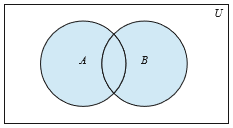
\includegraphics[scale=2]{chapter/imagens/31}
	\caption{Diagrama de Venn da união de $A$ e $B$.}
	\label{fig31}
\end{figure}

\begin{exmp}
\label{exem315}
A união dos conjuntos $\{1,3,5\}$ e $\{1,2,3\}$ é o conjunto $\{1,2,3,5\}$; isto
é, $\{1,3,5\} \cup \{1,2,3\} = \{1,2,3,5\}$.
\end{exmp}

\begin{defn}
\label{def311}
Sejam $A$ e $B$ dois conjuntos. A \emph{intersecção} dos conjuntos $A$ e $B$,
denotada por $A \cap B$, é o conjunto que contém os elementos que estão tanto em
$A$ como em $B$.
\end{defn}

Um elemento $x$ pertence a intersecção dos conjuntos $A$ e $B$ se e somente se
$x$ pertence a $A$ e $x$ pertence a $B$. Isto nos diz que,
\begin{center}
$A \cap B = \{x \mid x \in A \land x \in B\}$.
\end{center}

O diagrama de Venn apresentado na figura \ref{fig32} representa a intersecção
dos dois conjuntos $A$ e $B$. A zona sombreada que está entre ambos os círculos
representando os conjuntos $A$ e $B$ é a área que representa a intersecção de
$A$ e $B$.

\begin{figure}[H]
	\centering
	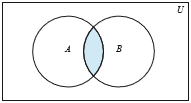
\includegraphics[scale=2.5]{chapter/imagens/32}
	\caption{Diagrama de Venn da intersecção de $A$ e $B$.}
	\label{fig32}
\end{figure}

\begin{exmp}
\label{exem316}
A intersecção dos conjuntos $\{1,3,5\}$ e $\{1,2,3\}$ é o conjunto $\{1,3\}$;
isto é $\{1,3,5\} \cap \{1,2,3\} = \{1,3\}$.
\end{exmp}

\begin{defn}
\label{def312}
Dois conjuntos são chamados de \emph{disjuntos} se a sua interseção é o conjunto
vazio (ou é nula).
\end{defn}

\begin{exmp}
\label{exem317}
Seja $A = \{1,3,5,7,9\}$ e $B = \{2,4,6,8,10\}$. Como $A \cap B = \emptyset$.
$A$ e $B$ são disjuntos.
\end{exmp}

Geralmente estamos interessados em encontrar a cardinalidade da união de dois
conjuntos finitos. Note que $|A| + |B|$ conta cada elemento em $A$ mas não em
$B$ ou em $B$ mas não em $A$ exactamente uma vez, e cada elemento que está em
ambos $A$ e $B$ é contado duas vezes. Assim, se o número de elementos que estão
ao mesmo tempo em $A$ e $B$ é subtraído de $|A|+|B|$, elementos em $A \cap B$
serão contados apenas uma vez. Dessa forma,
\begin{center}
$|A \cup B| = |A|+|B| - |A \cap B|$.
\end{center}

A generalização desse resultado para uniões de um número arbitrário de conjuntos
é chamado de \textbf{princípo de inclusão-exclusão}. Este princípio é
uma técnica importante utilizada em numeração.

Existem outras formas importantes de combinar dois conjuntos.

\begin{defn}
\label{def313}
Sejam $A$ e $B$ dois conjuntos. A \emph{diferença} entre $A$ e $B$, denotada por
$A - B$, é o conjunto que contém os elementos que existem em $A$ mas não existem
em $B$. A diferença entre $A$ e $B$ é também chamada de \emph{complemento} de
$B$ com respeito a $A$.
\end{defn}

\begin{description}
\item[Nota:] A diferença entre os conjuntos $A$ e $B$ é por vezes denotada por
$A\setminus B$.
\end{description}

Um elmento $x$ pertence a diferença entre $A$ e $B$ se e somente se $x \in A$ e
$x \notin B$. Isto nos diz que,
\begin{center}
$A - B = \{x \mid x \in A \land x \notin B\}$.
\end{center}

O diagrama de Venn apresentado na figura \ref{fig33} representa a diferença
entre os conjuntos $A$ e $B$.

\begin{figure}[H]
	\centering
	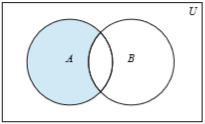
\includegraphics[scale=2]{chapter/imagens/33}
	\caption{Diagrama de Venn da diferença de $A$ e $B$.}
	\label{fig33}
\end{figure}

\begin{exmp}
\label{exem318}
A diferença entre $\{1,3,5\}$ e $\{1,2,3\}$ é o conjunto $\{5\}$; isto é,
$\{1,3,5\}-\{1,2,3\} = \{5\}$. Isto é diferente da diferença entre $\{1,2,3\}$ e
$\{1,3,5\}$, que é o conjunto $\{2\}$.
\end{exmp}

\begin{defn}
\label{def314}
Seja $U$ o conjunto universo. O complemento do conjunto $A$, denotado por
$\overline{A}$, é o complemento de $A$ com respeito a $U$. Assim, o complemento
do conjunto $A$ é $U - A$.
\end{defn}

Um elemento pertence a $\overline{A}$ se e somente se $x \notin A$. Isto nos diz
que,
\begin{center}
$\overline{A} = \{x \in U \mid x \notin A\}$.
\end{center}

Na figura \ref{fig34} a área sombreada fora do círculo que representa $A$ é a
área que representa $\overline{A}$.

\begin{figure}[H]
	\centering
	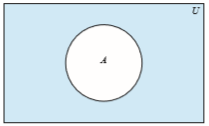
\includegraphics[scale=2]{chapter/imagens/34}
	\caption{Diagrama de Venn para o complemento de $A$.}
	\label{fig34}
\end{figure}


\begin{exmp}
\label{exem319}
Seja $A = \{a,e,i,o,u\}$, onde o conjunto-universo é o conjunto de todas as
letras do alfabeto, então $\overline{A} = \{b,c,d,f,g,h,j,\ldots,x,y,z\}$.
\end{exmp}

\begin{exmp}
\label{exem320}
Seja $A$ o conjunto dos números positivos inteiros maiores que 10 (onde o
conjunto universal é o conjunto de todos os positivos inteiros), então
$\overline{A} = \{1,2,3,4,5,6,7,8,9,10\}$.
\end{exmp}

\subsection*{\underline{Identidade de Conjuntos}}

A tabela \ref{tab:31} lista as identidades mais importantes dos conjuntos.
Iremos demonstrar algumas destas identidades utilizando três mêtodos diferentes.
Estes métodos são apresentados para ilustrar que geralmente existem diferentes
abordagens na resolução de um problema. As demonstrações das restantes
identidades serão deixadas como exercícios. Deverá notar também a similaridade
entre as identidades de conjuntos com as equivalências lógicas apresentadas no
capítulo \ref{cap:logicaformal}. Na verdade, as identidades de conjuntos
apresentadas podem demonstradas directamente das equivalências lógicas
correspondentes. Além disso, ambos são casos especiais de identidades da álgebra
de Boole.

\begin{table}[H]
	\centering
	\begin{tabular}{|l|l|}%
	\toprule
	\textbf{Identidade} & \textbf{Nome}\\
	\midrule
	$A \cap U = A$ &	Leis da Identidade\\
	$A \cup \emptyset = A$ &	\\
	\midrule
	$A \cup U = U$ &	Leis da Dominação\\
	$A \cap \emptyset = \emptyset$ &\\
	\midrule
	$A \cup A = A$ &	Leis da Idempotência\\
	$A \cap A = A$ &	\\
	\midrule
	$\overline{(\overline{A})} = A$ & Lei da Complementação\\
	\midrule
	$A \cup B = B \cup A$ & Leis Comutativas\\
	$A \cap B = B \cap A$ &\\
	\midrule
	$A \cup (B \cup C) = (A \cup B) \cup C$ & Leis Associativas\\
	$A \cap (B \cap C) = (A \cap B) \cap C$ &\\
	\midrule
	$A \cup (B \cap C) = (A \cup B) \cap (A \cup C)$ & Leis Distributivas
	\\
	$A \cap (B \cup C) = (A \cap B) \cup (A \cap C)$ & \\
	\midrule
	$\overline{A \cap B} = \overline{A} \cup \overline{B}$ & Leis de De Morgan\\
	$\overline{A \cup B} = \overline{A} \cap \overline{B}$ &\\
	\midrule
	$A \cup (A \cap B) = A$ & Leis da Absorção\\
	$A \cap (A \cup B) = A$&\\
	\midrule
	$A \cup \overline{A} = U$ & Leis do Complemento\\
	$A \cap \overline{A} = \emptyset$ &	\\
	\bottomrule%
	\end{tabular}%
	\caption{Idnetidades de conjuntos.}
	\label{tab:31}
\end{table}

Uma forma de demonstrar que dois conjuntos são iguais é por demonstrar que um é
subconjunto do outro e vice-versa. Lembre-se que para mostrar que um conjunto é
subconjunto de um outro conjunto, podemos mostrar que se um elemento pertence ao
primeiro conjunto então também deverá pertencer ao segundo conjunto. Geralmente
utilizamos uma demonostração directa para fazer isso. Iremos ilustrar este tipo
de demonstração por estabelecer a primeira lei de De Morgan.

\begin{exmp}
\label{exem321}
Demonstre que $\overline{A \cap B} = \overline{A} \cup \overline{B}$
\begin{description}
\item[Solução:] Iremos primeiramente demonstrar que os dois conjuntos
$\overline{A \cap B}$ e $\overline{A} \cup \overline{B}$ são iguais por provar
que cada um deles é subconjunto do outro. 

Primeiro, mostramos que $\overline{A \cap B} \subseteq \overline{A} \cup
\overline{B}$. Fazemos isto por provar que se $x$ está em $\overline{A \cap B}$,
então deverá também estar em $\overline{A} \cup \overline{B}$. Agora, suponha
que $x \in \overline{A \cap B}$. Pela definição do complemento, $x \notin A
\cap B$. Usando a definição de intersecção, vemos que a proposição $\lnot ((x
\in A) \land (x \in B))$ é verdadeira.

Ao aplicar a lei de De Morgan para as proposições, temos que $\lnot(x \in A)$ ou
$\lnot(x \in B)$. Utilizando a definição de negação das proposições, temos que
$x \notin A$ ou $x \notin B$. Utilizando a definição do complemento de um
conjunto, vemos que isto implica que $x \in \overline{A}$ ou $x \in
\overline{B}$. Consequentemente, pela definição da união, vemos que $x \in
\overline{A} \cup \overline{B}$. Temos agora demonstrado que $\overline{A
\cap B} \subseteq \overline{A} \cup \overline{B}$.

Agora, iremos mostrar que $\overline{A} \cup \overline{B} \subseteq
\overline{A \cap B}$. Fazemos isso por mostrar que se $x$ está em $\overline{A}
\cup \overline{B}$, então também deverá estar em $\overline{A \cap B}$. Suponha
agora que $x \in \overline{A} \cup \overline{B}$. Pela definição de união,
sabemos que $x \in \overline{A}$ ou $x \in \overline{B}$. Utilizando a definição
de complemento, vemos que $x \notin A$ ou $x \notin B$. Consequentemente, a
proposição $\lnot (x \in A) \lor \lnot (x \in B)$ é verdadeira.

Pela lei de De Morgan das proposições, concluímos que $\lnot ((x \in A) \lor
(x \in B))$ é verdadeira. Pela definição de intersecção, segue-se que $\lnot
(x \in A \cap B)$. Acabamos de utilizar a definição do complemento para concluir
que $x \in \overline{A \cap B}$. Isto mostra que $\overline{A} \cup
\overline{B} \subseteq \overline{A \cap B}$.

Como demonstramos que cada conjunto é subconjunto do outro, os dois conjuntos
são iguais e a identidade está provada.
\end{description}
\end{exmp}

Podemos agora mais sucintamente expressar este raciocínio no exemplo
\ref{exem321}, utilizando a notação de construção de domínios, tal como o
exemplo \ref{exem322} ilustra.

\begin{exmp}
\label{exem322}
Utilize a notação de construção de conjuntos e equivalências lógicas para
estabelecer a primeira lei de De Morgan $\overline{A \cap B} = \overline{A}
\cup \overline{B}$.
\begin{description}
\item[Solução:]Podemos provar esta identidade com os seguintes passos:

\begin{table}[H]
	\centering
	\begin{tabular}{rcll}%
	$\overline{A \cap B}$&$=$ & $\{x \mid x \notin A \cap B\}$ 			& \emph{pela
	definição do complemento}\\
	 					 &$=$ & $\{x \mid \lnot (x \in (A \cap B))\}$	& \emph{pela definição de
	 					 não pertença}\\
	 					 &$=$ & $\{x \mid \lnot (x \in A \land x \in B)\}$ & \emph{pela
	 					 definição de intersecção}\\
						 &$=$ & $\{x \mid \lnot(x \in A) \lor \lnot (x \in B)\}$ & \emph{pela
						 1a. lei de De Morgan para equivalências lógicas} \\
						 &$=$ & $\{x \mid x \notin A \lor x \notin B\}$ & \emph{pela definição de
						 não pertença}\\
						 &$=$ & $\{x \mid x \in \overline{A} \lor x \in \overline{B}\}$ &
						 \emph{pela definição do complemento}\\
						 &$=$ & $\{x \mid x \in \overline{A} \cup \overline{B}\}$ & \emph{pela
						 definição da união}\\
						 &$=$ & $\overline{A} \cup \overline{B}$ & \emph{pelo significado do
						 construtor de conjunto}			 
	\end{tabular}%
\end{table}
Note que para além das definições do complemento, união, pertença em conjuntos e
o construtor de conjuntos, esta demonstração utiliza a segunda lei de De Morgan
das equivalências lógicas.
\end{description}
\end{exmp}

\section{Funções}
\subsection*{\underline{Introdução}}

Em muitas instâncias atribuímos a cada elemento de um conjunto um outro elemento
particular de um segundo conjunto (que poderá ser o mesmo que o primeiro). Por
exemplo, suponha que a cada estudante na disciplina de Estruturas Discreta é
atribuído uma classificação do conjunto $\{10, 12, 13, 14, 17\}$.
Suponha também que estas notas são distribuídas a um grupo de alunos da seguinte
forma: 10 para o Aldo, 13 para a Carla, 12 para o Gabriel, 10 para a Rosa e 17
para o Samuel. Esta atribuição é ilustrada na figura \ref{fig35}.

\begin{figure}[H]
	\centering
 	\begin{tikzpicture}[ele/.style={fill=black,circle,minimum width=.8pt,inner
 sep=1pt}] 
 
 	\node[ele,label=left:Adão] (a1) at (0,5) {};    
  	\node[ele,label=left:Carla] (a2) at (0,4) {};    
	\node[ele,label=left:Gabriel] (a3) at (0,3) {};
	\node[ele,label=left:Rosa] (a4) at (0,2) {};
	\node[ele,label=left:Samuel] (a5) at (0,1) {};
	\node[ele,,label=right:10] (b1) at (4,5) {};
	\node[ele,,label=right:12] (b2) at (4,4) {};
	\node[ele,,label=right:13] (b3) at (4,3) {};
	\node[ele,,label=right:14] (b4) at (4,2) {};
	\node[ele,,label=right:17] (b5) at (4,1) {};
	%\node[draw,fit= (a1) (a2) (a3) (a4),minimum width=2cm] {} ;
	%\node[draw,fit= (b1) (b2) (b3) (b4),minimum width=2cm] {} ;  
	\draw[->,thick,shorten <=2pt,shorten >=2pt] (a1) -- (b1);
	\draw[->,thick,shorten <=2pt,shorten >=2] (a2) -- (b3);
	\draw[->,thick,shorten <=2pt,shorten >=2] (a3) -- (b2);
	\draw[->,thick,shorten <=2pt,shorten >=2] (a4) -- (b1);
 	\draw[->,thick,shorten <=2pt,shorten >=2] (a5) -- (b5);
 	\end{tikzpicture}
 	\caption{Atribuição de notas na disciplina de Estrutura Discretas.}
	\label{fig35}
\end{figure}

Esta atribuição é um exemplo de uma função. O conceito de função é extremamente
importante em matemática e ciência da computação. Por exemplo, em
matemática discreta, funções são utilizadas  na definição destas estruturas
discretas como sequências. Funções também são também utilizadas para representar
quanto tempo um computador leva para resolver um problema de um determinado
tamanho. Muitos programas de computadores e subrotinas de programação, são
desenhadas para calcular valores de funções. Funções recursivas, que são
funções definidas em termos de sí próprias, são utilizadas extensivamente em
ciência da computação.

\begin{defn}
\label{def315}
Sejam $A$ e $B$ dois conjuntos não-vazios. A \emph{função} $f$ de $A$ para $B$ é
uma atribuição de exactamente um elemento de $B$ a cada elemento de $A$.
Escrevemos $f(a) = b$ se $b$ é um único elemento de $B$ atribuído pela função
$f$ ao elemento $a$ de $A$. Se $f$ é uma função de $A$ para $B$, escrevemos
$f:A \to B$.
\end{defn}

\begin{description}
\item[Nota:]Funções são por vezes chamadas \textbf{mapeamentos} ou
\textbf{transformações}.
\end{description}

As funções são especificadas de várias formas. Por vezes nós apresentamos as
atribuições explicitamente, como na figura \ref{fig35}. Geralmente utilizamos
uma fórmula, como $f(x)=x+1$, para definir uma função. Noutras ocasiões
utilizamos um programa de computador para especificar uma função.

A função $f:A \to B$ pode ser também definida em termos de uma relação de $A$
para $B$. Uma relação de $A$ para $B$ é apenas um subconjunto de $A \times B$. A
relação de $A$ para $B$ que contém um, e apenas um, par ordenado $(a,b)$ para
cada elemento $a \in A$, define a função $f$ de $A$ para $B$. Esta função é
definida pela atribuição de $f(a)=b$, onde $(a,b)$ é o único par ordenado na
relação que possui $a$ como o seu primeiro elemento.

\begin{defn}
\label{def316}
Se $f$ é uma função de $A$ para $B$, dizemos que $A$ é o \emph{domínio} de $f$ e
$B$ é o co-domínio de $f$. Se $f(a)=b$, dizemos que $b$ é a \emph{imagem} de $a$
e $a$ é a pré-imagem de $b$. O \emph{alcance}, ou \emph{imagem}, de $f$ é o
conjunto de todas as imagens dos elementos de $A$. Também, se $f$ é uma função
de $A$ para $B$, dizemos que $f$ \emph{mapeia} $A$ em $B$.
\end{defn}

A figura \ref{fig36} representa a função $f$ de $A$ para $B$.

\begin{figure}[H]
	\centering
	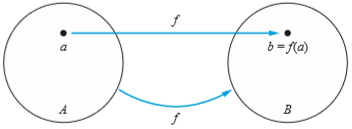
\includegraphics[scale=2]{chapter/imagens/36}
	\caption{Função $f$ que mapeia $A$ em $B$.}
	\label{fig36}
\end{figure}

Quando definimos uma função nós especificamos o seu domínio, co-domínio, e o
mapeamento dos elementos do domínio para os elementos no co-domínio. Duas
funções são \texbf{iguais} quando elas possuem o mesmo domínio, o mesmo
co-domínio, e mapeam cada elemento do domínio comum para os mesmos elementos do
co-domínio comum. Note que se mudarmos quer seja o domínio ou o co-domínio da
função, obteremos uma função diferente. Se mudarmos o mapeamento dos elementos,
obteremos também uma função diferente.

Os exemplos a seguir são exemplos de funções. Em cada exemplo, descrevemos o
domínio, o co-domínio, a imagem da função e a atribuição de valores para os
elementos do domínio.

\begin{exmp}
\label{exem323}
Seja $R$ a relação com os pares ordenados (André, 22), (Brenda, 24), (Carla,
21), (Doriel, 22), (Edna, 24) e (Felicia, 22). Cada um desses pares consiste no
nome de um estudante e a sua idade. Especifique uma função determinada por esta
relação?
\begin{description}
\item[Solução:]Se $f$ é a função especificada por $R$, então $f$(André) = 22,
$f$(Brenda) = 24, $f$(Carla) = 21, $f$(Doriel) = 22, $f$(Edna) = 24 e
$f$(Felicia) = 22. Aqui, $f(x)$ é a idade de $x$, onde $x$ é um estudante. Para
o domínio, temos o conjunto \{André, Brenda, Carla, Doriel, Edna, Felícia\}.
Precisamos também especificar o co-domínio, que deverá conter todas as idades
possíveis dos estudantes. Como é muito provável que os estudantes tenham todos
menos de 100 anos de idade, podemos indicar o conjunto dos números positivos
inteiros como o co-domínio. Note que poderíamos ter escolhido um co-domínio
diferente, como o conjunto dos inteiros positivos ou o conjunto dos inteiros
positivos entre 10 e 90, mas isto mudaria a função. Usar este co-domínio daria
também a possibilidade de extender a função por adicionar nomes e idades de mais
estudantes depois. A imagem da função especificada é o conjunto das diferentes
idades dos estudantes, que é o conjunto \{21,22,24\}.
\end{description}
\end{exmp}

\begin{exmp}
\label{exem324}
Seja $f$ a função que atribui os dois últimos bits de uma cadeia de bits de
tamanho 2 ou superior, a tal cadeia. Por exemplo $f(11010) = 10$. Assim, o
domínio de $f$ é o conjunto de todas as cadeias de bits de tamanho superior a 2,
e o co-domínio e a imagem são o conjunto $\{00,01,10,11\}$.
\end{exmp}

\begin{exmp}
\label{exem325}
Seja $f: \mathbf{Z} \to \mathbf{Z}$ que atribui o quadrado de um número inteiro
a este número. Então, $f(x) = x^2$, onde o domínio de $f$ é o conjuntos de
todos os números inteiros, o co-domínio de $f$ é o conjunto dos números
inteiros, e a imagem de $f$ é o conjunto de todos inteiros que são quadrados
perfeitos, nomeadamente, $\{0,1,4,9,\ldots\}$.
\end{exmp}

\begin{exmp}
\label{exem326}
O domínio e o co-domínio de funções geralmente são especificados em linguagens
de programação. Por exemplo, a seguinte expressão em Java
\begin{center}
\texttt{int piso (double num)\{\ldots\}}
\end{center}
nos diz que o domínio da função \texttt{piso} é o conjunto dos números
reais (representado pelo tipo de dados \texttt{double}) e o seu co-domínio é o
conjunto dos números inteiros.
\end{exmp}


\begin{defn}
\label{def317}
Sejam $f_1$ e $f_2$ funções de $A$ para $\mathbf{R}$. Então $f_1 + f_2$ e
$f_1f_2$ são também funções de $A$ para $\mathbf{R}$ definidas para todo $x \in
A$ por

\begin{center}
$(f_1+f_2)(x) = f_1(x) + f_2(x)$,\\
$(f_1f_2)(x) = f_1(x)f_2(x)$.
\end{center}

Note que as funções $f_1+f_2$ e $f_1f_2$ foram definidas pela especificação dos
seus valores em $x$ em termos dos valores de $f_1$ e $f_2$ em $x$.
\end{defn}

\begin{exemp}
\label{exem327}
Sejam $f_1$ e $f_2$ duas funções de $\mathbf{R}$ em $\mathbf{R}$ tal que
$f_1(x) = x^2$ e $f_2(x) = x - x^2$. Quais são os valores das funções $f_1 +
f_2$ e $f_1f_2$?
\begin{description}
\item[Solução:] Da definição da soma e produto de funções, temos que
\begin{center}
$(f_1 + f_2)(x) = f_1(x) + f_2(x) = x^2 + (x - x^2) = x$,
\end{center}
e
\begin{center}
$(f_1f_2)(x)=x^2(x-x^2) = x^3-x^4$.
\end{center}
\end{description}
\end{exemp}
Quando $f$ é uma função de $A$ para $B$, a imagem de um subconjunto de $A$
também pode ser definida.


\begin{defn}
\label{def318}
Seja $f$ uma função de $A$ para  $B$ e seja $S$ um subconjunto de $A$. A
\emph{imagem} de $S$ sobre a função $f$ é o subconjunto de $B$ que consiste nas
imagens dos elementos de $S$. Denotamos a imagem de $S$ por $f(S)$, tal que
\begin{center}
$f(S) = \{t \mid \exists s \in S (t = f(s))\}$.
\end{center}
Também podemos utilizar a notação curta $\{f(s) \mid s \in S\}$ para denotar
este conjunto
\begin{description}
\item[Nota:]A notação $f(S)$ para a imagem do conjunto $S$ sobre a função $f$ é
potencialmente ambígua. Aqui, $f(S)$ denota um conjunto e não o valor da função
$f$ no conjunto $S$.
\end{description}
\end{defn}

\begin{exmp}
\label{exem328}
Seja $A = \{a,b,c,d,e\}$ e $B=\{1,2,3,4\}$ com $f(a)=2$, $f(b)=1$, $f(c)=4$,
$f(d)=1$ e $f(e)=1$. A imagem do subconjunto $S=\{b,c,d\}$ é o conjunto
$f(S)=\{1,4\}$.
\end{exmp}


\subsection*{\underline{Funções injectivas e sobrejectivas}}

Algumas funções nunca atribuiem o mesmo valor para dois elementos diferentes do
domínio. Estas funções são chamadas de \texbf{injectivas}.

\begin{defn}
\label{def320}
A função $f$ é chamada de uma \emph{injunção}, se e somente se $f(a) = f(b)$
implica que $a=b$ para todo $a$ e $b$ no domínimo de $f$. A função é chamada de
\emph{injectiva} se for uma injunção.
\end{defn}

Note que um função $f$ é injectiva se e somente se $f(a) \neq f(b)$ sempre que
$a \neq b$. Esta forma de expressar que $f$ é uma injunção é obtida por obter a
contrapositiva da implicação na definição.

\begin{description}
\item[Nota:]Podemos expressar que $f$ é uma injunção utilizando quantificadores
como $\forall a\forall b (f(a)=f(b) \to a = b)$ ou equivalentemente $\forall
a\forall b(a \neq b \to f(a) \neq f(b))$, onde o universo em discurso é o
domínio da função.
\end{description}

Ilustraremos este conceito com alguns exemplos de funções que são injectivas e
outras que não são.

\begin{exmp}
\label{exem329}
Determine se a função $f$ de $\{a,b,c,d\}$ para $\{1,2,3,4,5\}$ com $f(a)=4$,
$f(b)=5$, $f(c)=1$ e $f(d)=3$ é injectiva.
\begin{description}
\item[Solução:]A função $f$ é injecetiva porque $f$ obtém valores diferentes nos
quatro elementos do seu domínio. Isto é ilustrado na figura \ref{fig37}.
\end{description}
\end{exmp}

 \begin{figure}[H]
	\centering
 	\begin{tikzpicture}[ele/.style={fill=black,circle,minimum width=.8pt,inner
 sep=1pt}] 
 
 	\node[ele,label=left:a] (a1) at (0,5) {};    
  	\node[ele,label=left:b] (a2) at (0,4) {};    
	\node[ele,label=left:c] (a3) at (0,3) {};
	\node[ele,label=left:d] (a4) at (0,2) {};
	\node[ele,,label=right:1] (b1) at (4,5) {};
	\node[ele,,label=right:2] (b2) at (4,4) {};
	\node[ele,,label=right:3] (b3) at (4,3) {};
	\node[ele,,label=right:4] (b4) at (4,2) {};
	\node[ele,,label=right:5] (b5) at (4,1) {};
	%\node[draw,fit= (a1) (a2) (a3) (a4),minimum width=2cm] {} ;
	%\node[draw,fit= (b1) (b2) (b3) (b4),minimum width=2cm] {} ;  
	\draw[->,thick,shorten <=2pt,shorten >=2pt] (a1) -- (b4);
	\draw[->,thick,shorten <=2pt,shorten >=2] (a2) -- (b5);
	\draw[->,thick,shorten <=2pt,shorten >=2] (a3) -- (b1);
	\draw[->,thick,shorten <=2pt,shorten >=2] (a4) -- (b3);
 	\end{tikzpicture}
 	\caption{Uma função injectiva.}
	\label{fig37}
\end{figure}

\begin{exmp}
\label{exem330}
Determine se a função $f(x)=x^2$ do conjunto dos números inteiros para o
conjunto dos números inteiros é injectiva.

\begin{description}
\item[Solução:]A função $f(x)=x^2$ não é injectiva porque, por exemplo,
$f(1)=f(-1)=1$, mas no entanto $1 \neq -1$.
Note que a função $f(x)=x^2$ com os seus domínios restrictos de \textbf{Z}$^+$ é
injectiva. (Tecnicamente, quando restringimos o domínio de uma função, obtemos
uma nova função cujos valores coincidem com os mesmo valores da função original
para os elementos do domínio restricto. A função restricta não é definida para
os elementos do domínio original fora do domínio restricto.)
\end{description}
\end{exmp}

\begin{exmp}
\label{exem331}
Determine se a função $f(x)=x+1$ do conjunto dos números reais para o mesmo
conjunto é injectiva.
\begin{description}
\item[Solução:]A função $f(x)=x+1$ é uma função injectiva. Para demonstrar isto,
note que $x+1 \neq y+1$ quando $x \neq y$.
\end{description}
\end{exmp}

\begin{defn}
\label{def321}
Uma função $f$ cujo domínio e co-domínio são subconjuntos do conjuntos dos
números reais é chamada de \emph{crescente} se $f(x) \leq f(y)$, e
\emph{estritamente crescente} se $f(x) < f(y)$, quando $x<y$ e $x$ e $y$ estão
no domínio de $f$.
Similarmente, $f$ é chamada de \emph{decrescente} se $f(x) \geq f(y)$, e
\emph{estritamente decrescente} se $f(x) > f(y)$, sempre que $x<y$ e $x$ e $y$
estão no domínio de $f$. (A palavra \emph{estritamente} nesta definição indica
que desigualdade.)
\end{defn}

\begin{description}
\item[Nota:]Uma função $f$ é crescente se $\forall x\forall y(x<y \to f(x) \leq
f(y))$, estritamente crescente se $\forall x\forall y(x<y \to f(x) < f(y))$,
decrescente se $\forall x\forall y(x<y \to f(x) \geq f(y))$ e estritamente
decrescente se $\forall x\forall y(x<y \to f(x) > f(y))$, onde o universo de
discurso é o domínio de $f$.
\end{description}

\begin{defn}
\label{def322}
A função $f$ de $A$ para $B$ é chamada de \emph{sobrejectiva}, se e somente se
para cada elemento $b \in B$ existe um elemento $a \in A$ com $f(a)=b$.

\begin{description}
\item[Nota:]A função $f$ é sobrejectiva se $\forall y\exists x(f(x)=y)$, onde o
domínio para $x$ é o domínio da função e o domínio para $y$ é o co-domínio da
função.
\end{description}
\end{defn}

\section{Matrizes (Opcional)}
\section{Sequências (Opcional)}%conjuntos, fun��es, matrizes e sequencias
\chapter*{Exercícios do Capítulo \ref{cap:conjuntos}}
%%1

\section*{Conjuntos}

\begin{enumerate}
  	\item Seja $A$ o conjunto dos estudantes que vivem à $5 km$ do campus e $B$ o conjunto dos estudantes que vêm 
  	de bicicleta às aulas. Descreva os estudantes em cada um dos seguintes conjuntos.
  	\begin{enumerate}
  	  	\item $A \cap B$ \item $A \cup B$ \item $A - B$ \item $B - A$
  	\end{enumerate}
  	
  	\item Liste os elementos dos seguintes conjuntos:
  	\begin{enumerate}
  		 \item $\{x | x \in \mathbb{N} \land x^2 < 25\}$ \item $\{x | x$ é um dos antigos vencedores da Fórmula 1 $\}$
  		 \item $\{x | x \in \mathbb{R} \land x^2 = -1\}$ \item $\{x | x \in \mathbb{N} \land x^2 - 5x + 6 = 0\}$
	\end{enumerate}
	
	\item Qual é cardinalidade de cada um dos seguintes conjuntos?
	\begin{enumerate}
	  	\item $ S = \{a, \{a, \{a\}\}\}$ \item $\{\{a\}, \{\{a\}\}\}$ \item $\{a, \{\emptyset \}, \emptyset\}$
	  	\item $\{\emptyset, \{\emptyset, \{\emptyset\}\},\{\emptyset, \{\emptyset, \{\emptyset\}\}\}\}$
	\end{enumerate}
	
  	\item Suponha que $A$ é o conjunto dos estudantes do segundo ano e $B$ é o conjunto dos estudantes de Lógica de Programação.
  	Descreva cada um dos conjuntos em termos de $A$ e $B$.
  	\begin{enumerate}
  		\item O conjunto dos estudantes do segundo ano com a cadeira de Lógica de Programação
  		\item O conjunto dos estudantes do segundo ano que não têm a cadeira de Lógica de Programação
  		\item O conjunto dos estudantes que são, ou do segundo ano ou têm a cadeira de Lógica de Programação
  		\item O conjunto dos estudantes que não são do segundo ano, nem têm a cadeira de Lógica de Programação
	\end{enumerate}

	\item Sejam, $A = \{a, b, c, d, e\}$ e $B = \{a, b, c, d, e, f, g, h\}$ encontre:
	\begin{enumerate}
	  \item $A \cup B$ \item $A \cap B$ \item $A - B$ \item $B - A$ 
	\end{enumerate}
	
	\item Desenhe os diagramas de Venn para cada uma das seguintes combinações dos domínios A, B e C
	\begin{enumerate}
		\item $A \cap (B \cup C)$ \item $A \cap B \cap C$ \item $(A - B) \cup (A - C) \cup (B - C)$ 
		\item $A \cap (B - C)$ \item $(A \cap B) \cup (A \cap C)$ \item $(A \cap B) \cup (A \cap C)$
	\end{enumerate}
\end{enumerate}

\newpage
\section*{Exercícios com Programação}

Escreva programas de computador com as entradas e saídas especificadas.
\begin{enumerate}
  \item Dados dois conjuntos finitos, liste todos os elementos do produto
  Cartesiano dos dois conjuntos.
  \item Dado um conjunto finito, liste todos os elementos do seu
  conjunto-potência.
  \item Dados dois conjuntos $A$ e $B$ subconjuntos do mesmo conjunto universal,
  encontre os conjuntos $A \cup B$, $A \cap B$ e $A - B$.
\end{enumerate}

\chapter*{Exercícios}
%%1
\section*{Funções}

\begin{enumerate}
	\item Determine se $f$ é uma função de $\mathbb{Z}$ em $\mathbb{R}$ se
	\begin{enumerate}
		\item $f(n) = \pm n$ \item $\sqrt{n^2 + 1}$ \item $\frac{1}{(n^2 - 4)}$  
	\end{enumerate}
	
	\item Determine se as seguintes funções de $\mathbb{Z}$ para $\mathbb{Z}$ são injectivas ou sobrejectivas.
	\begin{enumerate}
	  	\item $f(n) = n - 1$ \item $f(n) = n^2 + 1$ \item $f(n) = n^3$ \item $f(n) = \frac{n}{2}$
	\end{enumerate}
	
	\item Considere as seguintes funções do conjunto dos estudantes de Estruturas Discretas. Em que condições uma função é injectiva
	se ela atribui a um estudante o seu:
	\begin{enumerate}
	  	\item Número de telemóvel
	   	\item Número de estudante
	   	\item Nota final
	   	\item Local de Nascimento
	\end{enumerate}

	\begin{description}
		\item[Definição 1] Uma função diz-se \emph{bijectiva} quando é ao mesmo tempo injectiva (um para um) e sobrejectiva.
		\item[Exemplo 1] Seja $f$ uma função da forma $\{a,b,c,d\}$ para $\{1,2,3,4\}$ com $f(a) = 4, f(b) = 2, f(c) = 1$ e $f(d) = 3$.
		A função $f$ é uma função injectiva e sobrejectiva. É injectiva porque não existem valores no domínio que são mapeados
		para o mesmo valor no co-domínio. É sobrejectiva porque todos os quatro elementos do co-domínio são imagens dos elementos
		no domínio. Então $f$ é uma função \emph{bijectiva} ou uma \emph{bijeção}.	
	\end{description}
	
	\item Determina se cada uma das seguintes funções é uma bijeção de $\mathbb{R}$ para $\mathbb{R}$.
	\begin{enumerate}
		\item $f(x) = -3x + 4$ \item $f(x) = -3x^2 + 7$ \item $f(x) = (x+1)/(x+2)$ \item $f(x) = x^5 + 1$ \item $f(x) = 2x + 1$
		\item $f(x) = x^2 + 1$
	\end{enumerate}
	
	\begin{description}
		\item[Definição 2] Seja $f$ a função de $A$ para $B$ e seja $S$ um subconjunto de $A$. A imagem de $S$ sobre a função $f$ é o
		subconjunto de $B$ que consiste nas imagens dos elementos de $S$. Denotamos a imagem de $S$ por $f(S)$, tal que
		$f(S) = \{t | \exists s \in S(t = f(s))\}$. Também podemos utilizar a representação $\{f(s) | s \in S\}$
		\item[Exemplo 2] Seja $A = \{a,b,c,d,e\}$ e $B = \{1,2,3,4\}$ com $f(a)=2, f(b)=1, f(c)=4, f(d)=1$, e $f(e)=1$. A imagem
		do subconjunto $S = \{b,c,d\}$ é o conjunto $f(S) = \{1, 4\}$.
	\end{description}

	\item Seja $S = \{-1,0,2,4,7\}$ encontre $f(S)$ se
	\begin{enumerate}
	  	\item $f(x)=1$ \item $f(x)=2x + 1$ \item $f(x)=\lceil \frac{x}{5} \rceil$ \item $f(x) = \lfloor \frac{(x^2 + 1)}{3} \rfloor$  
	\end{enumerate}

	\item Seja $f(x) = \lfloor \frac{x^2}{3} \rfloor$, encontre $f(S)$ se,
	\begin{enumerate}
		\item $S = \{-2,-1,0,1,2,3\}$ \item $S=\{0,1,2,3,4,5\}$ \item $S=\{1,5,7,11\}$ \item $S=\{2,6,10,14\}$ 
	\end{enumerate}
	
	\item Seja $f: \mathbb{N} \to \mathbb{N}$ definida por $f(x) = x + 1$. Seja $g: \mathbb{N} \to \mathbb{N}$ definida por $g(x) = 3x$.
	Calcule o seguinte:
	\begin{enumerate}
	  	\item $(g \circ f)(5)$ \item $(f \circ g)(5)$ \item $(g \circ f)(x)$ \item $(f \circ g)(x)$ \item $(f \circ f)(x)$
	  	\item $(g \circ g)(x)$
	\end{enumerate}
	
	\item Para cada uma das seguintes bijeções $f: \mathbb{R} \to \mathbb{R}$, encontre $f^{-1}$
	\begin{enumerate}
	  	\item $f(x)=7x$ \item $f(x) = x^3$ \item $f(x) = \frac{(x + 4)}{3}$
	\end{enumerate}
\end{enumerate}

%\section*{Exercícios com programação}


\vspace*{2em}
\chapter{Relações}
\label{cap:relacoes}

Relações entre elementos de conjuntos ocorrem em muitos contextos. Todos dias
lidamos com relações como por exemplo: uma pessoa e o seu número de telemóvel,
um empregado(a) e o seu salário, etc. Em matemática estudamos relações como as
que existem entre um número inteiro positivo e um seu divisor, um inteiro e o
seu quadrado, um valor real $x$ e o valor $f(x)$ onde $f$ é uma função, etc.

As relações são representadas utilizando uma estrutura chamada de
\emph{relação}, que é simplesmente um subconjunto do produto cartesiano de
conjuntos. As relações podem ser utilizadas para resolver problemas tais como:
determinar quais pares de cidades estão ligadas pela mesma companhia área numa
rede, armazenamento de informações em bases de dados, etc.

\section{Relações e suas propriedades}

A forma mais directa de expressar uma relação entre elementos de dois conjuntos
é por utilizar pares ordenados (dois elementos). Por esta razão, os conjuntos de
pares ordenados são chamados de \emph{relações binárias}. Nesta secção
apresentamos a terminologia básica utilizada para descrever as relações binárias.

\label{def41}
\begin{defn}
Sejam $A$ e $B$ conjuntos, uma relação binária de $A$ para $B$ é um subconjunto
de $A \times B$.
\end{defn}

Por outras palavras, uma relação binária de $A$ para $B$ é um conjunto $R$ de
pares ordenados onde o primeiro elemento de cada par ordenado provém de $A$ e o
segundo elemento provém de $B$. Utilizamos a notação $a$ $R$ $b$ para denotar
que $(a,b) \in R$ e $a \centernot{R} b$ para denotar que $(a,b) \notin R$. Além
disso, quando $(a,b)$ pertecem a $R$, dizemos que $a$ \emph{está relacionado} à
$b$ por intermédio de $R$.

As relações binárias representam relacionamentos entre elementos de dois
conjuntos. Apresentaremos mais adiante as relações n-árias que expressam
relacionamentos entre elementos de mais de dois conjuntos. Iremos omitir a
palavra \emph{binária} sempre que não houver perigo de má interpretação. Os
exemplos a seguir ilustram o conceito de \emph{relação}.

\label{exem41}
\begin{exmp}
Sejam $A$ o conjunto dos estudantes da tua escola, e $B$ o conjunto das
disciplinas. Seja $R$ a relação que consiste nos pares $(a,b)$, onde $a$ é um
estudante inscrito na disciplina $b$. Por exemplo, se João e David estão
inscritos na disciplina de Estruturas Discretas (ED), os pares (João, ED) e
(David, ED) pertecem a $R$. Note que se David não está inscrito na disciplina de
ED, então o par (David, ED) não pertence a $R$. Se um estudante não está
inscrito em nenhuma disciplina, não existirá nenhum par em $R$ com este
estudante como primeiro elemento. Da mesma forma se uma disciplina não existe,
não existirá nenhum par em $R$ com esta disciplina como segundo elemento.
\end{exmp}

\label{exem42}
\begin{exmp}
Sejam  $A = \{0,1,2\}$ e $B = \{a,b\},$ então $\{(0,a), (0,b), (1,a), (2,b)\}$ é
uma relação de $A$ para $B$. Isto significa que, por exemplo, $0$ $R$ $a$, mas
$1 \centernot{R} b$.
\end{exmp}

\section{Relações sobre um conjunto}

\label{def42}
\begin{defn}
Uma \emph{relação} num conjunto $A$ é uma relação de $A$ para $A$.
\end{defn}

Por outras palavras, uma relação sobre um conjunto $A$ é um subconjunto de $A
\times A$.

\label{exem43}
\begin{exmp}
Seja $A$ o conjunto $\{1,2,3,4\}$. Que pares ordenados fazem parte da relação $R
= \{(a,b)$ | $a$ divide $b\}$?
	\begin{description}
	\item[Solução:]Como $(a,b)$ pertence a $R$ se e somente se $a$ e $b$ forem
	inteiros positivos não maiores que 4 tal que $a$ divida $b$, vemos que
	\[R=\{(1,1), (1,2), (1,3), (1,4), (2,2), (2,4), (3,3), (4,4)\}.\] Os pares
	nesta relação são apresentados graficamente e em forma tabular na Figura
	\ref{fig41}.
	\end{description}
\end{exmp}

\begin{figure}[H]
	\centering
	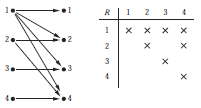
\includegraphics[scale=2.5]{chapter/imagens/41}
	\caption{Apresentando os pares ordenados na relação $R$ no exemplo
	\ref{exem43}.}
	\label{fig41}
\end{figure}

\label{exem44}
\begin{exmp}
Considere as seguintes relações no conjunto dos números inteiros:\\
	$R_1 = \{(a,b)$ | $a \leq b\}$,\\
	$R_2 = \{(a,b)$ | $a > b\}$,\\
	$R_3 = \{(a,b)$ | $a = b $ ou $ a = -b\}$,\\
	$R_4 = \{(a,b)$ | $a = b\}$,\\
	$R_5 = \{(a,b)$ | $a = b + 1\}$,\\
	$R_6 = \{(a,b)$ | $a + b \leq 3\}$,\\
	Qual destas relações contém cada um dos pares $(1,1), (1,2), (2,1), (1,-1)$ e
$(2,2)?$

\begin{description}
\item[Solução:]O par $(1,1)$ está em $R_1, R_3, R_4$ e $R_6$; $(1,2)$ está em
$R_1$ e $R_6$; $(2,1)$ está em $R_2, R_5$ e $R_6$;$(1,-1)$ está em $R_2, R_3$ e
$R_6$; e finalmente, $(2,2)$ está em $R_1, R_3$ e $R_4$.
\end{description}
\end{exmp}


\section{Propriedades das relações}
Existem várias propriedades que são utilizadas para classificar as relações
sobre um conjunto. Iremos apresentar as mais importantes de seguida.

Nalgumas relações um elemento está sempre relacionado consigo próprio. Por
exemplo, seja $R$ a relação no conjunto de todas as pessoas, consistindo nos pares
$(x,y)$ onde $x$ e $y$ são filhos da mesmo pai e da mesma mãe, então $x$ $R$ $y$
para todas as pessoas $x$.

\label{def43}
\begin{defn}
A relação $R$ num conjunto $A$ é chamada de \emph{reflexiva} se $(a,a) \in R$
para todo o elemento $a \in A$.
	
\begin{description}
\item[Nota:]Utilizando quantificadores vemos que uma relação $R$ num conjunto
$A$ é reflexiva se $\forall a((a,a) \in R)$, onde o universo em discurso é o
conjunto de todos os elementos em $A$.
\end{description}
\end{defn}

Vemos que a relação em $A$ é reflexiva se todo elemento de $A$ está relacionado
consigo próprio. Os exemplos a seguir ilustram o conceito de uma relação
reflexiva.

\label{exem45}
\begin{exmp}
Considere as seguintes relações em $\{1,2,3,4\}$:
	\begin{itemize}
		\item $R_1 = \{(1,1),(1,2),(2,1),(2,2),(3,4),(4,1),(4,4)\},$
		\item $R_2 = \{(1,1),(1,2),(2,1)\},$
		\item $R_3 = \{(1,1),(1,2),(1,4),(2,1),(2,2),(3,3),(4,1),(4,4)\},$
		\item $R_4 = \{(2,1),(3,1),(3,2),(4,1),(4,2),(4,3)\},$
		\item $R_5 = \{(1,1),(1,2),(1,3),(1,4),(2,2),(2,3),
		(2,4),(3,3),(3,4),(4,4)\},$
		\item $R_6 = \{(3,4)\}.$
	\end{itemize}
	Quais destas relações são reflexivas?
	
\begin{description}
\item[Solução:]As relações $R_3$ e $R_5$ são reflexivas porque ambas contêm
todos os pares na forma $(a,a)$, nomeadamente, $(1,1), (2,2), (3,3)$ e $(4,4)$.
As outras relações não são reflexivas porque não contêm todos estes pares
ordenados. Em particular $R_1, R_2, R_4$ e $R_6$ não são reflexivas porque
por exemplo $(3,3)$ não faz parte de nenhuma destas relações.
\end{description}
\end{exmp}

\label{exem46}
\begin{exmp}
	Quais das relações no exemplo \ref{exem45} são reflexivas?
	\begin{description}
	\item[Solução:]As relações reflexivas do exemplo \ref{exem45} são $R_1$ (porque
	$a \leq a$ para todo inteiro $a$), $R_3$ e $R_4$. Para cada uma das outras
	relações no exemplo citado é fácil encontrar um par da forma $(a, a)$ que não
	faz parte de nenhuma das relações.
	\end{description}
\end{exmp}

\label{def44}
\begin{defn}
	A relação $R$ num conjunto $A$ é chamada de \emph{simétrica} se $(b,a) \in R$
	sempre que $(a,b) \in R$, para todos $a, b \in A.$ A relação $R$ num conjunto
	$A$ tal que para todo $a,b \in A$, se $(a,b) \in R$ e $(b,a) \in R$, então $a =
	b$, é chamada de \emph{antissimétrica}.
	
	\begin{description}
	\item[\emph{Nota:}]Utilizando quantificadores vemos que uma relação $R$ num
	conjunto $A$ é simétrica se $\forall{a}\forall{b}((a,b) \in R \to (b,a) \in
	R))$. Similarmente, a relação $R$ num conjunto $A$ é antissimétrica se
	$\forall{a}\forall{b}(((a,b) \in R \land (b,a) \in R) \to (a = b)).$
	\end{description}
\end{defn}


Tenha em atenção que uma relação é simétrica se e somente se $a$ está
relacionado à $b$ implica que $b$ está relacionado à $a$. A relação é
antissimétrica se e somente se não existírem pares de distintos elementos $a$ e
$b$ com $a$ relacionado a $b$ e $b$ relacionado a $a$. Isto é, a única forma de
ter $a$ relacionado à $b$ e $b$ relacionado a $a$ é se $a$ e $b$ forem os mesmos
elementos. Os termos \emph{simétrica} e \emph{antissimétrica} não são opostos,
porque a relação pode ter ambas propriedades ou não. A relação só não pode ser
ao mesmo tempo simétrica e antissimétrica se contém algum par da forma $(a,b),$
onde $a \centernot{=} b$.

\label{exem47}
\begin{exmp}
Quais das relações no exemplo \ref{exem45} são simétricas e quais são
antissimétricas?

\begin{description}
\item[Solução:]As relações $R_2$ e $R_3$ são simétricas, porque em
cada caso $(b,a)$ pertence a relação sempre que $(a,b)$ está na relação. Para
$R_2$, a única coisa a verificar é se ambos $(2,1)$ e $(1,2)$ estão na relação.
Para $R_3$, é necessário verificar que $(1,2)$ e $(2,1)$ pertencem a relação, e
$(1,4)$ e $(4,1)$ pertencem a relação. Pode-se facilmente verificar que as
outras relações não são simétricas. Isto pode ser feito por encontrar um par
$(a,b)$ na relação para o qual não exista um par $(b,a)$. $R_4, R_5$ e $R_6$ são
todas antissimétricas. Para cada uma destas relações não existe um par de
elementos $a$ e $b$ com $a \centernot{=} b$ tal que ambos $(a,b)$ e $(b,a)$
pertencem a relação. O leitor pode verificar que nenhuma das outras relações é
antissimétrica. Isto pode ser feito por encontrar um par $(a,b)$ com $a
\centernot{=} b$ tal que $(a,b)$ e $(b,a)$ estão ambos na relação.
\end{description}
\end{exmp}

\label{def45}
\begin{defn}
A relação $R$ num conjunto $A$ é chamada de \emph{transitiva} se sempre que
$(a,b) \in R$ e $(b,c) \in R$, então $(a,c) \in R$, para todos $a, b, c \in
A$.

\begin{description}
\item[\emph{Nota:}]Utilizando quantificadores vemos que uma relação $R$ num
conjunto $A$ é transitiva se temos $\forall{a}\forall{b}\forall{c}(((a,b) \in R
\land (b,c) \in R) \to (a,c) \in R)$.
\end{description}
\end{defn}

\label{exem48}
\begin{exmp}
Quais das relações no exemplo \ref{exem45} são transitivas?

\begin{description}
\item[Solução:]As relações $R_4, R_5$ e $R_6$ são transitivas. Para cada uma
destas relações, poderemos provar que são transitivas por verificar que se
$(a,b)$ e $(b,c)$ pertencem a esta relação, então $(a,c)$ também fazem parte.
Por exemplo, $R_4$ é transitiva, porque $(3,2)$ e $(2,1)$, $(4,2)$ e $(2,1)$,
$(4,3)$ e $(3,1)$, e $(4,3)$ e $(3,2)$ fazem parte da relação tal como os pares
$(3,1),(4,1)$ e $(4,2)$. Como exercício, verifique se $R_5$ e $R_6$ são
transitivas. $R_1$ não é transitiva porque $(3,4)$ e $(4,1)$ pertencem a $R_1$,
mas $(3,1)$ não. $R_2$ não é transitiva porque $(2,1)$ e $(1,2)$ pertencem a
$R_2$, mas $(2,2)$ não fazem parte. $R_3$ não é transitiva porque $(4,1)$ e
$(1,2)$ pertencem a $R_3$, mas $(4,2)$ não.
\end{description}
\end{exmp}


	
\section{Combinação de relações}

Como as relações de $A$ para $B$ são subconjuntos de $A \times B$, duas
relações de $A$ para $B$ podem ser combinadas da mesma forma como os conjuntos
podem ser combinados. Considere os exemplos abaixo:

\label{exem49}
\begin{exmp}
Sejam $A = \{1,2,3\}$ e $B = \{1,2,3,4\}$. As relações $R_1 = \{(1, 1), (2, 2),
(3, 3)\}$ e $R_2 = \{(1, 1), (1, 2), (1, 3), (1, 4)\}$ podem ser combinadas
para obter:
\begin{itemize}
	\item $R_1 \cup R_2 = \{(1, 1), (1, 2), (1, 3), (1, 4), (2, 2), (3, 3)\}$
	\item $R_1 \cap R_2 = \{(1,1)\}$
\end{itemize}
\end{exmp}

\label{exem410}
\begin{exmp}
Seja $R_1$ a relação ``menor que'' no conjunto dos números reais e seja $R_2$ a
relação ``maior que'' no conjunto dos números reais, isto é, $R_1 = \{(x,y)
\mid x < y\}$ e $R_2 = \{(x,y) \mid x > y\}$. O que são $R_1 \cup R_2$, $R_1
\cap R_2$, $R_1 - R_2$ e $R_2 - R_1$?

\begin{description}
\item[\emph{Solução:}]Notamos que $(x,y) \in R_1 \cup R_2$ se e somente se
$(x,y) \in R_1$ ou $(x,y) \in R_2$. Assim, $(x,y) \in R_1 \cup R_2$ se e somente
se $x < y$ ou $x > y$. Como a condição $x < y$ ou $x > y$ é o mesmo que a
condição $x \neq y$, segue-se que $R_1 \cup R_2 = \{(x,y) \mid x \neq y\}$. Por
outras palabras, a união da relação ``menor que'' com a relação ``maior que'' é
a relação ``diferente de''.
De seguida, note que é impossível para um par $(x,y)$ pertencer a ambos os pares
$R_1$ e $R_2$ porque é impossível que $x<y$ e $x>y$. Segue-se que $R_1 \cap R_2
= \emptyset$. Também notamos que $R_1 - R_2 = R_1$ e $R_2 - R_1 = R_2$.
\end{description}
\end{exmp}

Existe uma outra forma de combinar relações que é análoga a composição de
funções.

\label{def46}
\begin{defn}
Seja $R$ a relação de um conjunto $A$ para um conjunto $B$ e $S$ uma relação de
$B$ para $C$. A \emph{composta} de $R$ e $S$ é a relação que consiste nos pares
ordenados $(a,c)$, onde $a \in A$, $c \in C$ e para os quais existe um elemento
$b \in B$ tal que $(a,b) \in R$ e $(b,c) \in S$. Denotamos a composta de $R$ e
$S$ por $S \circ R$.
\end{defn}

Calcular a composta de duas relações requer que encontremos elementos que são o
segundo elemento de um par ordenado na primeira relação e o primeiro elemento de
pares ordenados na segunda relação, como os exemplos a seguir ilustram.

\label{exem411}
\begin{exmp}
Qual é a composta das relaçãoes $R$ e $S$, onde $R$ é a relação de $\{1,2,3\}$
para $\{1,2,3,4\}$ com $R = \{(1,1),(1,4),(2,3),(3,1),(3,4)\}$ e $S$ é uma
relação de $\{1,2,3,4\}$ para $\{0,1,2\}$ com $S =
\{(1,0),(2,0),(3,1),(3,2),(4,1)\}$?

\begin{description}
\item[\emph{Solução:}] $S \circ R$ é construída utilizando todos os pares
ordenados em $R$ e pares ordenados em $S$, onde o segundo elemento do par
ordenado em $R$ é o mesmo que o primeiro elemento do par ordenado em $S$. Por
exemplo, os pares ordenados $(2,3)$ em $R$ e $(3,1)$ em $S$ produzem o par
ordenado $(2,1)$ em $S \circ R$. Computando todos os pares ordenados na composta
de $S$ e $R$ obtemos,
\begin{center}
$S \circ R = \{(1,0), (1,1), (2,1), (2,2), (3,0), (3,1)\}$.
\end{center}
\end{description}
\end{exmp}


\label{exem412}
\begin{exmp}
\textbf{Compondo uma relação consigo própria} Seja $R$ a relação no conjunto de
todas as pessoas tal que $(a,b) \in R$ se a pessoa $a$ é o pai da pessoa $b$.
\end{exmp}



\section{Representação de relações}

\subsection{Introdução}

\textbf{Nota}: Nesta secção, utilizaremos sómente as relações binárias. Por
esta razão a palavra relação irá apenas referir-se a relações binárias.

Existem muitas formas de representar uma relação entre conjuntos finitos. Uma
forma é por listar os pares ordenados.
Outra forma de representar uma relação é por meio de tabelas como vimos na
secção anterior. Nesta secção vamos apresentar dois métodos de representação
alternativos: matrizes zero-um e gráfos direccionados. No geral, as matrizes
são apropriadas para a representação de relações em programas de computador.
Por outro lado, algumas pessoas acham a representação de relações utilizando
grafos direccionados mais útil ao entendimento das propriedades dessas relações.

\subsection{Representação de relações por meio de matrizes}

A relação entre conjuntos finitos pode ser representada utilizando matrizes
zero-um. Suponha que $R$ é uma relação de $A = \{a_1, a_2, \ldots, a_m\}$ para
$B = \{b_1, b_2, \ldots, b_n\}$. (Aqui os elementos dos conjuntos A e B são
listados duma forma particular, embora arbitrária. Além dos mais, quando $A =
B$ utilizamos a mesma ordenação para $A$ e $B$.) A relação $R$ pode ser
representada pela matriz $M_R = [m_{ij}]$,\\


$m_{ij} = \begin{cases}
	1$ se $(a_i, b_j) & \in R,\\
	0$ se $(a_i, b_j) & \notin R.
\end{cases}$


Por outras palavras, a matriz zero-um que representa $R$ tem o valor 1 em
$(i,j)$ quando $a_i$ está relacionado a $b_j$, e o valor 0 nesta posição se
$a_i$ não está relacionado a $b_j$. Esta representação depende da ordem
utilizada para $A$ e $B$. A utilização de matrizes para representar relações é
ilustrada no exemplos a seguir.

\begin{description}
	\elabel{exe610}
	\item[Exemplo \ref{exe610}] {Suponha que $A = \{1,2,3\}$ e $B = \{1,2\}$. Seja
	R a relação de $A$ para $B$ contendo os pares $(a,b)$ se $a \in A$, $b \in B$
	e $a > b$. Qual é a matriz que representa $R$ se $a_1 = 1$, $a_2 = 2$, $a_3 =
	3$ e $b_1 = 1$ e $b_2 = 2?$}
\end{description}

\emph{Solução:} Como $R = \{(2, 1), (3, 1), (3, 2)\}$, a matriz para $R$ é:

\[
M_R = \begin{bmatrix}
	0 & 0\\
	1 & 0\\
	1 & 1
\end{bmatrix}
\]

Os 1s em $M_R$ mostram que os pares $(2,1), (3,1)$ e $(3,2)$ pertencem a $R$. Os 0s mostram que os outros pares não
pertencem a $R$.

\begin{description}
	\elabel{exe611}
	\item[Exemplo \ref{exe611}]{Sejam $A = \{a_1, a_2, a_3\}$ e $B = \{b_1, b_2,
	b_3, b_4, b_5\}$, quais pares ordenados estão na relação $R$ representada pela
	matriz}
\end{description}

\[
	M_R = \begin{bmatrix}
	0 & 1 & 0 & 0 & 0\\
	1 & 0 & 1 & 1 & 0\\
	1 & 0 & 1 & 0 & 1
	\end{bmatrix}?
\]
	
\emph{Solução} Como $R$ consiste nos pares ordenados $(a_i, b_j)$ com $m_{ij} =
1$ daí resulta que $R = \{(a_1,b_2), (a_2,b_1), (a_2, b_3), (a_2, b_4), (a_3,
b_1), (a_3, b_3), (a_3, b_5)\}$

A matriz de uma relação em um conjunto, que é uma matriz quadrada, pode ser
utilizada para determinar se a relação possui certas propriedades. Sabemos que
uma relação $R$ num conjunto $A$ é reflexiva se $(a,a) \in R$ sempre que $a \in
A$, então, $R$ é reflexiva se e somente se $(a_i, a_i) \in R$ para $i =
1,2,\ldots,n$. Assim, $R$ é reflexiva se e somente se $m_{ii} = 1$, para $i =
1,2,\ldots,n$. Por outras palavras, $R$ é reflexiva se todos os elementos da
diagonal principal de $M_R$ são iguais a $1$, como ilustrado na Figura
\ref{Figura61}. Note que os elementos fora da diagonal podem ser $0s$ ou $1s$.

\begin{figure}[H]
	\centering
	\[
	\begin{bmatrix}
	 1	& 	& 	&	&	&	&	&\\
	 	& 1 &	&	&	&	&	&\\
		&	& 1 &	&	&	&	&\\
		&	&  	& .	&	&	&	&\\
		&	&	& 	& . &	&	&\\
		&	&	&	&	& . &	&\\
		&	&	& 	&	&	& 1	&\\
		&	&	&	&	&	&	& 1 
	\end{bmatrix}
	\]
	\caption{A matriz zero-um para uma relação reflexiva. (Os elementos fora da diagonal podem ser 0 ou 1.)}
	\label{Figura61}
\end{figure}

A relação $R$ é simétrica se $(a,b) \in R$ implica que $(b, a) \in R$.
Consequentemente, a relação $R$ no conjunto $A = \{a_1, a_2, \ldots, a_n\}$ é
simétrica se e somente se $(a_j, a_i) \in R$ sempre que $(a_i, a_j) \in R$. Em
termos dos valores de $M_R$, $R$ é simétrica se e somente se $m_{ji} = 1$
sempre que $m_{ij} = 1$. Isto também significa que $m_{ji} = 0$ sempre que
$m_{ij} = 0$. Consequentemente, $R$ é simétrica se e somente se $m_{ij} =
m_{ji}$, para todos os pares de inteiros $i$ e $j$ com $i = 1,2,\ldots,n$ e
$j=1,2,\ldots,n$. $R$ é simétrica se e somente se $M_R = (M_R)^t$ onde
$(M_R)^t$ é matriz transposta de $M_R$.

A relação $R$ é antissimétrica se e somente se $(a, b) \in R$ e $(b, a) \in R$
implica que $a = b$. Consequentemente, a matrix de uma relação antissimétrica
tem a propriedade de que se $m_{ij} = 1$ com $i \ne j$, então $m_{ji} = 0$.
Ou, em outras palavras, $m_{ij} =0$ ou $m_{ji} =0$ quando $i \ne j$. A forma da
matriz para uma relação antissimétrica é ilustrada na Figura \ref{Figura62}.

\begin{figure}[H]
	\centering
	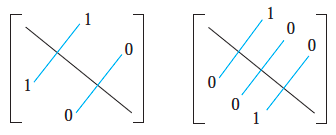
\includegraphics[scale=0.6]{chapter/imagens/62}
	\caption{A matriz zero-um para uma relação simétrica e antissimétrica.}
	\label{Figura62}
\end{figure}

\begin{description}
	\elabel{exe612}
	\item[Exemplo \ref{exe612}]{Suponha que a relação $R$ é representada pela
	matriz}
\end{description}
\[
	M_R = \begin{bmatrix}
	1 & 1 & 0\\
	1 & 1 & 1\\
	0 & 1 & 1
	\end{bmatrix}?
\]

$R$ é reflexiva, simétrica e/ou antisimétrica?

\emph{Solução:} Como todos os elementos das diagonais nesta matriz são iguais a
$1$, $R$ é reflexiva.
Além do mais, como $M_R$ é simétrica, então $R$ é simétrica. É também fácil
notar que $R$ não é antissimétrica.

As operações booleanas estudadas anteriormente também podem ser utilizadas para
encontrar as matrizes que representam a união e a intersecção de duas relações.
Suponha que $R_1$ e $R_2$ são relações num conjunto $A$ representada pelas
matrizes $M_{R_1}$ e $M_{R_2}$, respectivamente. A matriz que representa a
união destas duas relações possui o valor $1$ nas posições em que  $M_{R_1}$ ou
$M_{R_2}$ possuem o valor $1$. A matriz que representa a intersecção destas
duas relações possui o valor $1$ nas posições em que  $M_{R_1}$ e $M_{R_2}$
possuem o valor $1$.
Sendo assim, as matrizes que representam a união e a intersecção destas duas
relações são:

\begin{itemize}
  \item $M_{R_1 \cup R_2} = M_{R_1} \lor M_{R_2}$ e,
  \item $M_{R_1 \cap R_2} = M_{R_1} \land M_{R_2}$
\end{itemize}


\subsection{Representação de relações por meio de grafos direccionados}

Vimos anteriormente que uma relação pode ser representada por uma listagem de
todos os seus pares ordenados ou por meio de uma matriz zero-um. Existe outra
forma importante de representar uma relação utilizando uma representação
pictural. Cada elemento do conjunto é representado por um ponto, e cada par
ordenado é representado utilizando um arco cuja direcção é indicada por uma
seta.
Utilizamos essa representação sempre que pensamos em relações como grafos
direccionados ou dígrafos, num conjunto finito.


\begin{description}
	\dlabel{def66}
	\item[Definição \ref{def66}]{Um \emph{grafo direccionado}, ou \emph{dígrafo},
	consiste num conjunto $V$ de \emph{vértices} (ou \emph{nós}) e um conjunto $E$
	de pares ordenados dos elementos de $V$ chamados de \emph{arestas} (ou
	\emph{arcos}). O vértice $a$ é chamado de \emph{vértice inicial} da aresta
	$(a,b)$, e o vértice $b$ é chamado de \emph{vértice terminal} desta aresta.}
\end{description}

Uma aresta da forma $(a, a)$ é representada utilizando um arco do vértice $a$ de volta à sí mesmo. Tal aresta é chamada de 
\textbf{laço} ou \textbf{loop}.


\begin{description}
	\elabel{exe613}
	\item[Exemplo \ref{exe613}]{O grafo direccionado com os vértices $a, b, c$ e
	$d$ e as arestas \\$(a,b), (a,d), (b,b), (b,d), (c,a), (c,b)$ e $(d,b)$ é
	apresentado na Figura \ref{Figura63}}
\end{description}

\begin{figure}[H]
	\centering
	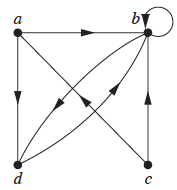
\includegraphics[scale=0.6]{chapter/imagens/63}
	\caption{Um grafo direccionado.}
	\label{Figura63}
\end{figure}


A relação $R$ no conjunto $A$ é representada pelo grafo ordenado que possui
elementos de $A$ como seus vértices e os pares ordenados $(a,b)$, onde $(a,b)
\in R$, como arestas. Esta atribuição configura uma correspondência
\emph{um-para-um} entre as relações no conjunto $A$ e os grafos direcionados que
possuem $A$ como o seu conjunto de vértices. Assim, cada afirmação sobre relações corresponde a
uma afirmação sobre grafos direccionados, e vice-versa. Grafos direccionados
fornecem uma exibição visual das relações e por isso são utilizados no estudo
das relações e de suas propriedades. A utilização de grafos direccionados na
represetntação de relações num conjunto é ilustrada nos seguintes exemplos.

\begin{description}
	\elabel{exe614}
	\item[Exemplo \ref{exe614}]{
	O grafo direccionado da relação\\
	$R = {(1, 1), (1, 3), (2, 1), (2, 3), (2, 4), (3, 1), (3, 2), (4, 1)}$\\
	no conjunto $\{1, 2, 3, 4\}$ é ilustrado na Figura \ref{Figura64}
	}
\end{description}

\begin{figure}[H]
	\centering
	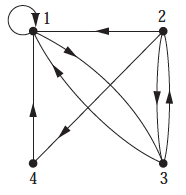
\includegraphics[scale=0.6]{chapter/imagens/64}
	\caption{Um grafo direccionado.}
	\label{Figura64}
\end{figure}

\begin{description}
	\elabel{exe615}
	\item[Exemplo \ref{exe615}]{
	Quais são os pares ordenados na relação $R$ representada pelo grafo direccionado da Figura \ref{Figura65}}
\end{description}

\begin{figure}[H]
	\centering
	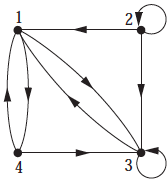
\includegraphics[scale=0.6]{chapter/imagens/65}
	\caption{Um grafo direccionado da relação R.}
	\label{Figura65}
\end{figure}

\emph{Solução:} Os pares ordenados $(x,y)$ na relação são \[$R = {(1,
3), (1, 4), (2, 1), (2, 2), (2, 3), (3, 1), (3, 3), (4, 1), (4, 3)}\]

Cada um destes pares corresponde à uma aresta do grafo direccionado sendo
$(2,2)$ e $(3,3)$ dois laços.

O grafo direccionado que representa uma relação pode ser utilizado para
determinar se a relação possui certas propriedades.
Por exemplo, a relação é reflexiva se e somente se existe um laço em cada
vértice do grafo direccionado, de tal forma que todos os pares ordenados da
forma $(x,x)$ ocorrem na relação. A relação é simétrica se e somente se para
cada aresta entre vértices distintos no digrafo existe uma aresta na direcção
oposta, tal que $(y,x)$ existe na relação sempre que $(x,y)$ existe na relação.
Da mesma forma, uma relação é antissimétrica se e somente se não existem duas
arestas em direcções opostas entre vértices distintos. Finalmente, uma relação
é transitiva se e somente se sempreque que existe uma aresta de um vértice $x$
para um vértice $y$ e uma aresta de um vértice $y$ para um vértice $z$, existe
uma aresta de $x$ para $z$ (completando um triângulo onde cada lado é uma aresta
na direcção correcta).


\begin{description}
	\elabel{exe616}
	\item[Exemplo \ref{exe616}]{Determine se os grafos direccionados apresentados
	nas Figuras \ref{Figura66} e \ref{Figura67} são reflexivos, simétricos,
	antissimétricos e/ou transitivos}.
\end{description}

\begin{figure}[H]
	\centering
	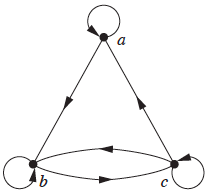
\includegraphics[scale=0.6]{chapter/imagens/66}
	\caption{Um grafo direccionado da relação R.}
	\label{Figura66}
\end{figure}

\begin{figure}[H]
	\centering
	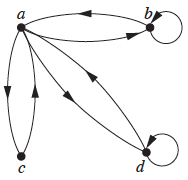
\includegraphics[scale=0.6]{chapter/imagens/67}
	\caption{Um grafo direccionado da relação S.}
	\label{Figura67}
\end{figure}

\emph{Solução:} Como existem laços em todos os vértices do grafo direccionado
de $R$, ele é reflexivo. $R$ não é simétrico nem anti-simétrico porque existe
uma aresta de $a$ para $b$ mas não de $b$ para $a$, mas existem arestas em
ambas direcções que conectam $b$ e $c$. Finalmente, $R$ não é transitivo porque
existe uma aresta de $a$ para $b$ e uma aresta de $b$ para $c$, mas não existe
uma aresta de $a$ para $c$. Como não existem laços em todos os vértices do grafo
direccionado de S, esta relação não é reflexiva. É simétrica mas não
antissimétrica, porque cada aresta entre vértices distintos é acompanhada por
uma aresta na direcção oposta. Não é díficil notar também que o grafo
direccionado de $S$ não é transitivo, porque $(c,a)$ e $(a,b)$ pertencem a $S$,
mas $(c,b)$ não pertence a $S$.

Estudaremos os grafos em mais detalhes no capítulo \ref{cap:grafos}.


\section{Fecho de relações (Opcional)}

\subsection{Introdução}

Uma rede de computadores de uma empresa possui centros de dados em Benguela,
Bengo, Cabinda, Cunene, Huíla e Luanda.
Existem ligações directas de Benguela para o Bengo, de Benguela para o Bengo,
de Benguela para Cunene, do Bengo para o Cunene, de Cunene para Cabinda e da
Huíla para Luanda. Seja $R$ a relação que contém $(a,b)$ se existe uma ligação
do centro de dados em $a$ com o centro de dados em $b$, como podemos determinar
se existe uma ligação (possívelmente indirecta) composta de uma ou mais linhas
de um centro para outro? Como nem todas as ligações são directas, tal como a
ligação de Benguela para Cabinda que passa por Cunene, $R$ não pode ser
utilizada directamente para responder esta questão.
Na linguagem das relações, $R$ não é transitiva, portanto não contém todos os
pares que podem ser ligado. Tal como iremos mostrar nesta secção, é possível
achar todos os pares de centros de dados que possuem um link por construír uma
relação transitiva $S$ que contém $R$ tal que $S$ é um subconjunto de todas as
relações transitivas que contêm $R$.


\section{Relações de equivalência}

\section{Ordens parciais (Opcional)}%relacoes
\chapter*{Exercícios}
%%1

\section*{Relações e suas propriedades}

\begin{enumerate}
  	\item {Liste os pares ordendados na relação $R$ de $A = \{0,1,2,3,4\}$ para $B = \{0,1,2,3\}$ onde $(a,b) \in R$ se
  	e somente se}
  	\begin{enumerate}
  	  	\item $a = b$ \item $a + b = 4$ \item $a > b$ \item $a | b$ \item $mdc(a,b)=1$ \item $mmc(a,b)=2$
  	\end{enumerate}
  	
  	\item{Para cada uma das relações no conjunto $\{1,2,3,4\}$ indiqye se são: reflexivas, simétricas, antissimétricas
  	e transitivas}
  	\begin{enumerate}
  	  	\item $\{(2, 2), (2, 3), (2, 4), (3, 2), (3, 3), (3, 4)\}$
  	  	\item $\{(1, 1), (1, 2), (2, 1), (2, 2), (3, 3), (4, 4)\}$
  	  	\item $\{(2, 4), (4, 2)\}$
  	  	\item $\{(1, 2), (2, 3), (3, 4)\}$
  	  	\item $\{(1, 1), (2, 2), (3, 3), (4, 4)\}$
  	  	\item $\{(1, 3), (1, 4), (2, 3), (2, 4), (3, 1), (3, 4)\}$
  	\end{enumerate}

  	\item {Determine se a relação $R$ conjunto de todas as pessoas é reflexiva, simétrica, antissimétrica, e/ou
  	transitiva, onde $(a,b) \in R$ se e somente se}
  	\begin{enumerate}
  		\item $a$ é mais alto que $b$.
  		\item $a$ e $b$ foram nascidos no mesmo dia.
  		\item $a$ possui o mesmo apelido que $b$.
  		\item $a$ e $b$ possuem o mesmo avó.
  	\end{enumerate}	
\end{enumerate}

%\section*{Representação de relações}

%\section*{Exercícios com programação}

\vspace*{2em}
\chapter{Grafos}
\label{cap:grafos}

Grafos são estruturas discretas que consistem em vértices, e arestas que
conectam estes vértices. Existem vários tipos de grafos, dependendo da
existência de uma direcção nas arestas, de acordo a possibilidade de várias
arestas se interligarem ao mesmo par de vértices e de acordo a existência de
\emph{loops} ou repetições.
Problemas em quase todas as disciplinas podem resolvidos utilizando modelos de
grafos. Iremos apresentar alguns exemplos para ilustrar como os grafos são
utilizados como modelos numa variedade de aéras. Por exempo, iremos mostrar como
os grafos são utilizados para representar a competição de diferentes espécias
num nicho ecológico, e como os grafos são usados para representar quem
influencia quem numa organização e etc.

Utilizando modelos de grafos, podemos determinar se é possível caminhar todas as
ruas de uma cidade sem psasar por uma rua duas vezes, e podemos determinar o
número de cores necessário para colorar as regiões de um mapa. Grafos podem ser
utilizados para determinar se um circuito pode ser implementado numa placa de
circuitos plana. Podemos distinguir entre dois compostos químicos com a mesma
fórmula molecular mas estruturas diferentes utilizando grafos. Podemos
determinar se dois computadores estão conectados por um \emph{link} de
comunicação utilizando modelos gráficos de redes. Grafos com pesos atribuidos as
suas arestas podem ser utilizados para resolver problemas como encontrar o
caminho mais curto entre duas cidades numa rede de transporte. Neste capítulo
iremos apresentar os conceitos básicos da teoria dos grafos e apresentar alguns
modelos de grafos. Para resolver uma boa parte dos problemas que podem ser
estudados utilizando grafos, iremos apresentar alguns algoritmos de grafos.
Iremos também estudar a complexidade destes algoritmos.

\section{Grafos e Modelos de Grafos}

Começamos com a definição de grafos.
\begin{defn}
\label{def51}
Um \emph{grafo} $G = (V,E)$ consiste em $V$, um conjunto não-vazio de
\emph{vértices} (ou \emph{nós}) e $E$, um conjunto de \emph{arestas}. Cada
aresta possui ou um ou mais vértices associados a esta, chamada de sua
\emph{extremidade}. Diz-se que uma aresta \emph{conecta} as suas extremidades.
\end{defn}

\begin{description}
\item[\emph{Nota}:] O conjunto de vértices $V$ de um grafo $G$ pode ser
infinito. Um grago com um conjuntos infinito de vértices ou um
número infinito de arestas é chamado de \textbf{grafo infinito}, e em comparação, um grafo com
um conjunto de finito de vértices e um conjunto finito de arestas é chamado de
\textbf{grafo finito}. Neste manual iremos considerar apenas grafos finitos.
\end{description}

Agora imagine que uma rede de computadores é formada por centros de dados e
\textit{links} de comunicação entre computadores. Podemos representar a
localização de cada centro de dados por um ponto e cada \textit{link} de
comunicação por um segmento de linha, como mostra a Figura \ref{fig51}

\begin{figure}[H]
	\centering
	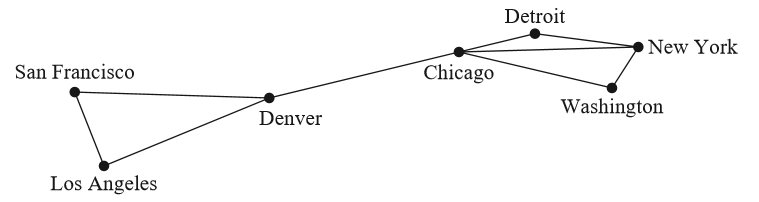
\includegraphics[scale=1]{chapter/imagens/51}
	\caption{Uma Rede de Computadores.}
	\label{fig51}
\end{figure}

Esta rede de computadores pode ser modelada utilzando grafos em que os vértices
do grafo representam centros de dados e as areas representam os \textit{links}
de comunicação. No geral, visualizamos os grafos usando pontos para represtentar
os vértices e segmentos de linha, possivelmente curvos, para representar as
arestas, onde as extremidades de um segmento de linha representando uma aresta
são os pontos representando as extremidades da aresta. Quando desenhamos um
grafo, geralmente tentamos desenhar as arestas de formas a não se cruzarem. No
entanto, isto não é necessário porque qualquer representação utilizando pontos
para representar os vértices e qualquer forma de conexão entre os vértices pode
ser utilizada. De facto, existem alguns grafos que não podem ser desenhados no
plano sem que as arestas se cruzem (veja a Secção \ref{sec:107}). O ponto
principal é que a forma como desenhamos um grafo é arbritária, desde que as
conexões correctas entre os vértices estejam representadas.

Note que cada aresta do grafo representando esta rede de computadores conecta
dois vértices diferentes. Isto é, nenhuma aresta conecta um vértice a si
próprio. Além disso, duas arestas diferentes não conectam o mesmo par de
vértices. Um grafo em que cada aresta conecta dois vértices diferentes e em que
duas arestas conectam o mesmo par de vértices é chamada de \textbf{grafo
simples}. Note que num grafo simples, cada aresta está associada à um par
não-ordenado de vértices, e mais nenhuma aresta está associada a esta mesma
aresta. Consequentemente, quando existe uma aresta de um grafo simples associada
a $\{u,v\}$, também podemos dizer, sem possibilidade de confusão, que $\{u,v\}$
é uma aresta do grafo.

Uma rede de computadores pode conter múltiplas ligações entre centros de dados,
como ilustrado na Figura \ref{fig52}. Para modelar tais redes precisamos de
grafos que posuam mais de uma aresta conectando o mesmo par de vértices. Grafos
que possam ter \textbf{múltiplas arestas} a conectar os mesmos vértices são
chamados de \textbf{multigrafos}. Quando existem $m$ arestas diferentes
associadas ao mesmo par não-ordenado de vértices $\{u,v\}$, também dizemos que
$\{u,v\}$ é uma aresta de multiplicidade $m$. Isto é, podemos pensar neste
conjunto de arestas como $m$ diferentes cópias de uma aresta $\{u,v\}$.

\begin{figure}[H]
	\centering
	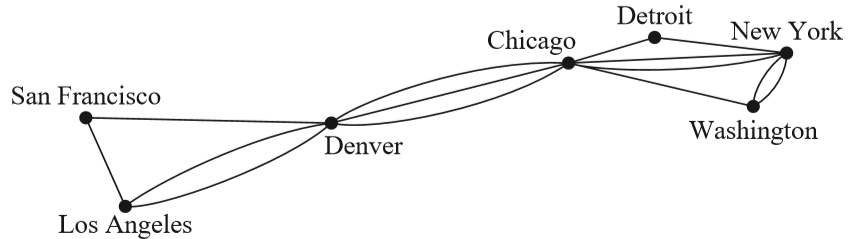
\includegraphics[scale=1]{chapter/imagens/52}
	\caption{Uma Rede de Computadores com Múltiplos LInks entre Centros de Dados.}
	\label{fig52}
\end{figure}

Por vezes um \textit{link} de comunicação de conecta um centro de dados consigo
próprio, possivelmente um laço de realimentação para diagnóstico. Uma rede deste
tipo é ilustrada na Figura \ref{fig53}. Para modelar esta rede precisamos
incluir arestas que conectem um vértice consigo próprio. Tais arestas são
chamadas de \textbf{laços} e as vezes podemos até ter mais de um laço no
vértice. Grafos que podem incluir laços, e possivelmente múltiplas arestas
conectando o mesmo par de vértices ou um vértice consigo próprio, são por vezes
chamados de \textbf{pseudo-grafos}.

\begin{figure}[H]
	\centering
	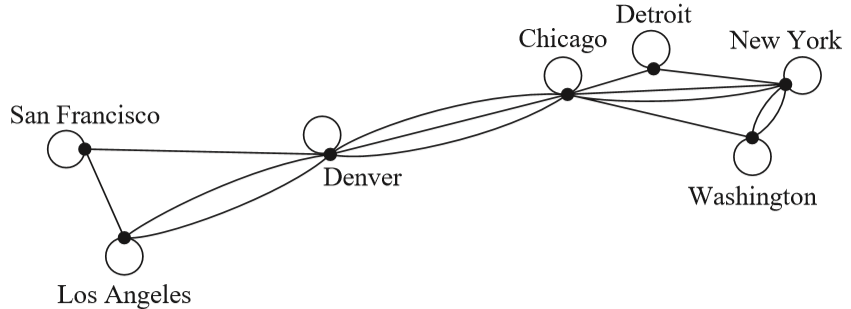
\includegraphics[scale=1]{chapter/imagens/53}
	\caption{Uma Rede de Computadores com Links para Diagnósticos.}
	\label{fig53}
\end{figure}


Até agora os grafos que apresentamos são \textbf{grafos não-direccionados}. As
suas arestas também são chamadas de \textbf{não direccionadas}. No entanto, para
construir um modelo de grafo, talvez achemos necessário atribuir direcções às
arestas do grafo. Por exemplo, numa rede de computadores, alguns \emph{links}
poderão operar apenas em uma direcção (tais ligaçõs são chamadas de linhas
\emph{duplex} simples). Isto pode ser o caso quando existe uma quantidade enorme
de tráfego enviada para alguns centros de dados, com pouco ou nenhum tráfego na
direcção oposta.

Para modelar tais redes de computadores utilizamos um grafo direccionado. Cada
aresta de um grafo direccionado está associada à um par ordenado. A definição de
um grafo direccionado que apresentamos aqui é mais geral do que a utilizada no
Capítulo \ref{cap:relacoes}, onde utilizamos grafos direccionados para
representar relações.

\begin{defn}
\label{def52}
Um \emph{grafo direccionado} (ou \emph{digrafo}) $(V,E)$ consiste num conjunto
não-vazio de vértices $V$ e um conjunto de \emph{arestas direccionadas} (ou
\emph{arcos}) $E$. Cada aresta direccionada está associada à um par ordenado de
vértices. A aresta direccionada associada ao par ordenado $(u,v)$ é dita que
\emph{começa} em $u$ e \emph{termina} em $v$.
\end{defn}

Quando representamos um grafo direccionado por meio de linhas, podemos utilizar
uma seta a apontar de $u$ à $v$ para indicar a direcção de uma aresta que começa
em $u$ e termina em $v$. Um grafo direccionado pode conter laços e pode conter
múltiplas arestas direccionadas que começam e terminam nos mesmos vértices. Um
grafo direccionado pode também conter arestas direccionads que conectam os
vértices $u$ e $v$ em ambas direcções; isto é, quando o dígrafo contém uma
aresta de $u$ à $v$, pode também conter uma ou mais arestas de $v$ para $u$.
Note que obtemos um grafo direccionado quando atribuímos uma direcção a cada
aresta em um grafo não-direccionado. Quando um grafo direccionado não possui
laços e não possui múltiplas arestas direccionadas, é chamado de \textbf{grafo
direccionado simples}. Como um grafo direccionado simples possui no máximo uma
aresta associada à cada par ordenado de vértices $(u,v)$, chamamos $(u,v)$ de
uma aresta se existe uma aresta associada à si no grafo.

Em algumas redes de computadores, multiplas ligações de comunicação entre dois
centros de dados podem ser representadas, como ilustrado na figura \ref{fig54}.
Grafos direccionados que possam ter \textbf{múltiplas arestas direccionadas} de
um vértice para outro vértice (possivelmente o mesmo) são usados para modelar
tais redes. Chamamos tais grafos de \textbf{multigrafos direccionados}. Quando
existm $m$ arestas direccionadas, cada associada à um par ordenado de vértices
$(u,v)$, dizemos que $(u,v)$ é uma aresta de \textbf{multiplicidade} $m$.

\begin{figure}[H]
	\centering
	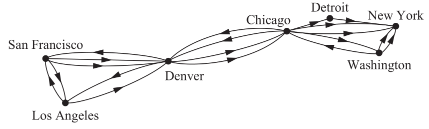
\includegraphics[scale=2]{chapter/imagens/54}
	\caption{Uma Rede de Computadores Múltiplos Links de Uma Via.}
	\label{fig54}
\end{figure}

Para alguns modelos podemos necessitar um grafo onde algums arestas não são
direccionadas, enquanto que outras são direccionadas. Um grafo com ambas arestas
direccionadas e não-direccionadas é chamado de \textbf{grafo misto}. Por
exemplo, um grafo misto pode ser utilizado para modelar uma rede de computadores
que contém ligações que operam em ambas direcções e outras ligações que operam
apenas em uma direcção.

Esta terminologia para os vários tipos de grafos é sumarizada na Tabela
\ref{tab51}. Iremos algumas vezes utilizar o termo \textbf{grafo} como um termo
deral para descrever grafos com arestas direccionadas ou não direccionadas (ou
ambos), com ou sem laços e com ou sem arestas múltiplas. Em outros casos, quando
o contexto estiver claro, iremos utilizar o termo grafo para nos referirmos
apenas aos grafos não-direccionados.

\begin{table}[H]
\centering
\begin{tabular}{|l|l|l|l|}%
\toprule
\textbf{Tipo} & \textbf{Arestas} & \textbf{Múltiplas Arestas?} &
\textbf{Laços?}
\\
\midrule
Grafo simples & Não direccionada & Não & Não \\
Multigrafo & Não direccionada & Sim & Não \\
Pseudo-grafo & Nao direccionada & Sim & Sim \\
Grafo direccionado simples & Direccionada & Não & Não \\
Multigrafo direccionado & Direccionada & Sim & Sim \\
Grafo misto & Direccionada e& Sim & Sim\\
&  \qquad não direccionada & &\\
\bottomrule%
\end{tabular}%
\caption{Terminologia dos Grafos.}
\label{tab51}
\end{table}

Por causa do recente interesse na teoria dos gradfos, e por causa da sua
aplicação à uma variedade de disciplinas, muitas terminologias da teoria dos
grados foram introduzidas. O estudante deverá determinar como tais termos estão
a ser utilizados quando os encontrar na literatura. A terminologia utilizada por
matemáticas para descrever grafos tem sido padronizada incrementalmente, mas a
terminologia usada em outras disciplinas ainda é muito variada. Embora a
terminologia usada para descrever grafos pode variar, três questões nos ajudam a
entender a estrutura de um grafo:
\begin{itemize}
  \item As arestas do grafo são não-direccionadas ou direccionadas (ou ambas)?
  \item Se o grafo é não-direccionado, existem múltiplas arestas que conectam o
  mesmo par de vértices? Se o grafo é direccionado, existem múltiplas arestas
  direccionads?
  \item Existem laços?
\end{itemize}

Responder a estas questões ajuda-nos a entender grafos independemente da
terminologia particular utilizada.


\subsection*{\underline{Modelos de Grafos}}

\begin{description}
\item[REDES SOCIAIS]
\item[REDES DE COMUNICAÇÃO]
\item[REDES DE INFORMAÇÃO]
\item[APLICAÇÕES PARA O DESENHO DE SOFTWARE]
\item[REDES DE TRANSPORTE]
\item[REDES BIOLÓGICAS]
\item[TORNEIOS]
\end{description}

\section{Terminologia dos Grafos e Tipos de Grafos Especiais}
\subsection*{\underline{Introdução}}
\subsection*{\underline{Terminologia Básica}}
\subsection*{\underline{Alguns Grafos Simples Especiais}}
\subsection*{\underline{Grafos Bipartidos}}
\subsection*{\underline{Grafos Bipartidos e Combinações}}
\subsection*{\underline{Algumas Aplicações dos Tipos de Grafos Especiais}}
\subsection*{\underline{Novos Grafos à Partir de Grados Antigos}}

\section{Representação de Grados e Isomorfismo de Grafos}
\subsection*{\underline{Introdução}}
\subsection*{\underline{Representação de Grafos}}
\subsection*{\underline{Matrizes de Adjacência}}
\subsection*{\underline{Matrizes de Incidência}}
\subsection*{\underline{Isomorfismo de Grafos}}
\subsection*{\underline{Determinando se Dois Grafos Simples são Isomórficos}}

\section{Conectividade}
\subsection*{\underline{Introdução}}
\subsection*{\underline{Trajectória}}
\subsection*{\underline{Conectividade de Grafos Não-Direccionados}}
\subsection*{\underline{O Quão Conectado é Um Grafo}}
\subsection*{\underline{Conectividade de Grafos Direccionados}}
\subsection*{\underline{Trajectória e Isomorfismo}}
\subsection*{\underline{Contando a Trajectória entre Vértices}}

\section{Trajectória de Euler e de Hamilton}

\section{Problemas do Caminho-Mais-Curto}

\section{Grafos Planares}

\section{Coloração de Grafos}









%grafos
\chapter*{Exercícios do Capítulo \ref{cap:grafos}}
%%1

\section*{Grafos}
\chapter{Árvores}%arvores
\chapter*{Exercícios}
%%1

\section*{Árvores}

%\chapter*{Consideraçõres finais}

\end{document}